% ថ្នាក់ទី ១១ (វិទ្យាសាស្ត្រសង្គម) · ជំពូកទី ៣ · មេរៀនទី ១ · សៀវភៅ ទំព័រ ៦៩–៨៩
\chapter{អនុគមន៍ត្រីកោណមាត្រ}

នៅថ្នាក់ទី $10$ យើងបានសិក្សារួចមកហើយពីអនុគមន៍ពហុធា ដូចជា $y = au$, $y = au^2$, $y = au^3 \ldots$ ដែលអនុវត្តក្នុងចលនាស្មើឬទន្លាក់សេរី ។ នៅថ្នាក់ទី $11$ នេះ យើងនឹងសិក្សាពីចលនាមួយទៀត ដូចចលនារំយោលនៃប៉ោលនាឡិកាមួយជាចលនាខួប ។ ចលនានេះគេសិក្សានៅក្នុងអនុគមន៍ត្រីកោណមាត្រជាអនុគមន៍ខួប ដូចជា អនុគមន៍ស៊ីនុស អនុគមន៍កូស៊ីនុស និងអនុគមន៍តង់សង់ ។

\begin{note}[ជំពូកទី ៣ ៖ អនុគមន៍ត្រីកោណមាត្រ]
ជំពូកនេះមានមេរៀន ៖ \textbf{១. អនុគមន៍ត្រីកោណមាត្រ} \quad \textbf{២. រូបមន្តត្រីកោណមាត្រ} \quad \textbf{៣. អនុគមន៍ច្រាសនៃអនុគមន៍ត្រីកោណមាត្រ} \quad \textbf{៤. សមីការនិងវិសមីការរូបមន្តត្រីកោណមាត្រ} ។
\end{note}

\begin{objBox}[វត្ថុបំណង]
\begin{enumerate}[1]
  \item បំប្លែងមុំពីដឺក្រេទៅរ៉ាដ្យង់និងពីរ៉ាដ្យង់ទៅដឺក្រេ
  \item ប្រើលក្ខណៈមុំផ្តុំក្នុងការគណនាអនុគមន៍ត្រីកោណមាត្រ
  \item សង់ក្រាបនៃអនុគមន៍ត្រីកោណមាត្រ ។
\end{enumerate}
\end{objBox}

\section{រង្វាស់មុំ}

\subsection{ការកំណត់មុំមានទិសដៅ}

\begin{example}[ឧទាហរណ៍ ១]
ក្នុងរង្វង់ត្រីកោណមាត្រ គេប្រើវ៉ិចទ័រ $\overrightarrow{OP_0}$ និង $\overrightarrow{OP}$ មកកំណត់មុំ ។

$\overrightarrow{OP_0}$ ជាវ៉ិចទ័រនឹងឋិតនៅផ្នែកវិជ្ជមាននៃអ័ក្ស $\overrightarrow{Ox}$ ហៅថា \textbf{វ៉ិចទ័រគល់} ។ $\overrightarrow{OP}$ ជាវ៉ិចទ័រចល័តជុំវិញគល់ $O$ ហៅថា \textbf{វ៉ិចទ័រចុង} ។

វ៉ិចទ័រ $\overrightarrow{OP_0}$ និង $\overrightarrow{OP}$ បង្កើតបានមុំតាមករណីដូចខាងក្រោម ៖
\begin{itemize}
  \item ក្នុងករណីវ៉ិចទ័រ $\overrightarrow{OP}$ វិលច្រាសនឹងទិសដៅនៃទ្រនិចនាឡិកា មុំដែលបង្កើតបានជាមុំវិជ្ជមាន ។ មុំ $(\overrightarrow{OP_0}, \overrightarrow{OP}) = 30^\circ$ (រូប ក) ។
  \item ក្នុងករណីវ៉ិចទ័រ $\overrightarrow{OP}$ វិលស្របនឹងទិសដៅនៃទ្រនិចនាឡិកា មុំដែលបង្កើតបានជាមុំអវិជ្ជមាន ។ មុំ $(\overrightarrow{OP_0}, \overrightarrow{OP}) = -30^\circ$ (រូប ខ) ។
\end{itemize}
\begin{center}
\begin{tikzpicture}[scale=0.9,>=stealth]
  \begin{scope}
    \draw[->] (-1.6,0) -- (1.7,0) node[right] {$x$};
    \draw[->] (0,-1.6) -- (0,1.7) node[above] {$y$};
    \draw[blue!70!black,thick] (0,0) circle (1.2);
    \draw[->,thick] (0,0) -- (30:1.2) node[above right] {$P$};
    \node[below right] at (1.2,0) {$P_0$};
    \node[below left] at (0,0) {$0$};
    \draw[->] (0.6,0) arc (0:30:0.6) node[midway,right] {\scriptsize $30^\circ$};
    \node at (0,-2) {រូប ក};
  \end{scope}
  \begin{scope}[xshift=4.5cm]
    \draw[->] (-1.6,0) -- (1.7,0) node[right] {$x$};
    \draw[->] (0,-1.6) -- (0,1.7) node[above] {$y$};
    \draw[blue!70!black,thick] (0,0) circle (1.2);
    \draw[->,thick] (0,0) -- (-30:1.2) node[below right] {$P$};
    \node[above right] at (1.2,0) {$P_0$};
    \node[above left] at (0,0) {$0$};
    \draw[->] (0.6,0) arc (0:-30:0.6) node[midway,right] {\scriptsize $-30^\circ$};
    \node at (0,-2) {រូប ខ};
  \end{scope}
\end{tikzpicture}
\end{center}
\end{example}

\begin{example}[ឧទាហរណ៍ ២]
តាមទិសដៅវិជ្ជមានបើ $\overrightarrow{OP}$ វិលបានមួយជុំពេញនៃរង្វង់នោះ គេនឹងបានមុំ $360^\circ$ ហើយរង្វាស់មុំនឹងកើនជា $2$ ដង ជា $3$ ដង ទៅតាមចំនួនជុំនៃការវិលនេះ ។
\begin{center}
\begin{tikzpicture}[scale=0.75,>=stealth]
  \foreach \k/\lab in {0/{1 ជុំ $= 360^\circ$},1/{2 ជុំ $= 2 \times 360^\circ$},2/{3 ជុំ $= 3 \times 360^\circ$}} {
    \begin{scope}[xshift=\k*4.6cm]
      \draw[->] (-1.7,0) -- (1.8,0) node[right] {$x$};
      \draw[->] (0,-1.7) -- (0,1.8) node[above] {$y$};
      \draw[blue!70!black,thick] (0,0) circle (1.3);
      \node at (0,-2.2) {\lab};
    \end{scope}}
  \draw[->,dashed] (0.3,0) arc (0:358:0.3);
  \begin{scope}[xshift=4.6cm]
    \draw[->,dashed] (0.3,0) arc (0:360:0.3) arc (0:358:0.5);
  \end{scope}
  \begin{scope}[xshift=9.2cm]
    \draw[->,dashed] (0.3,0) arc (0:360:0.3) arc (0:360:0.55) arc (0:358:0.8);
  \end{scope}
\end{tikzpicture}
\end{center}
\end{example}

បើ $\alpha$ ជាមុំកំណត់ដោយវ៉ិចទ័រ $\overrightarrow{OP_0}$ និង $\overrightarrow{OP}$ នោះ $\overrightarrow{OP_0}$ និង $\overrightarrow{OP}$ ក៏កំណត់មុំដែលមានរង្វាស់ផ្សេងៗគ្នាដូចខាងក្រោម ៖
\[
\begin{array}{ll}
\alpha + 360^\circ & \alpha - 360^\circ\\
\alpha + 2 \times 360^\circ & \alpha - 2 \times 360^\circ\\
\alpha + 3 \times 360^\circ & \alpha - 3 \times 360^\circ
\end{array}
\]

\begin{formulaBox}[ជាទូទៅ]
$\overrightarrow{OP_0}$ និង $\overrightarrow{OP}$ ជាពីរវ៉ិចទ័រកំណត់បានមុំ $\alpha + k360^\circ$, $k \in \mathbb{Z}$ ។
\end{formulaBox}

\begin{note}[សម្គាល់]
មុំ $\alpha$ និង $\alpha + 360^\circ$ មានរង្វាស់ខុសគ្នា ប៉ុន្តែមានវ៉ិចទ័រគល់និងវ៉ិចទ័រចុងដូចគ្នា ។
\end{note}

\begin{example}[លំហាត់គំរូ ១]
វ៉ិចទ័រ $\overrightarrow{OP}$ វិលចេញពីទីតាំងដើម $\overrightarrow{OP_0}$ បានមុំ $120^\circ$ ហើយបន្ទាប់មកវិលបានមុំ $-155^\circ$ ទៀត ។ ចូរកំណត់មុំ $(\overrightarrow{OP_0}, \overrightarrow{OP})$ ។
\end{example}
\ans
មុំ $(\overrightarrow{OP_0}, \overrightarrow{OP}) = 120^\circ + (-155^\circ) = -35^\circ$ ។

\begin{example}[លំហាត់គំរូ ២]
គណនាមុំ $\alpha = 45^\circ + k \times 360^\circ$ ក្នុងករណី $k = 1$, $k = -1$ ។
\end{example}
\ans
ចំពោះ $k = 1$, \ $\alpha = 45^\circ + 360^\circ = 405^\circ$ ។

ចំពោះ $k = -1$, \ $\alpha = 45^\circ - 360^\circ = -315^\circ$ ។

\begin{pro}
\begin{enumerate}[1]
  \item បើវ៉ិចទ័រ $\overrightarrow{OP}$ ផ្តើមវិលពីទីតាំងដើម $\overrightarrow{OP_0}$ បានមុំ $70^\circ$ តាមទិសដៅអវិជ្ជមាន ហើយបន្ទាប់មកវិលបានមុំ $150^\circ$ តាមទិសដៅវិជ្ជមាន ។ ចូរកំណត់មុំ $(\overrightarrow{OP_0}, \overrightarrow{OP})$ ។
  \item គណនា $\alpha = -270^\circ + k \times 360^\circ$ ក្នុងករណី $k = 2$, $k = -3$ ។
\end{enumerate}
\ans
\begin{enumerate}[1]
  \item $80^\circ$ ។
  \item $\alpha = 450^\circ$, \ $-1350^\circ$ ។
\end{enumerate}
\end{pro}

\subsection{រង្វាស់មុំគិតជារ៉ាដ្យង់}

\begin{example}[ឧទាហរណ៍]
រង្វង់មួយមានកាំ $r = 5$ cm និង $\angle AOB = 30^\circ$ ។ គណនាប្រវែងធ្នូ $AB$ ។ មុំផ្ចិតគិតជាដឺក្រេពុំមានទំនាក់ទំនងទៅនឹងប្រវែងធ្នូ $AB$ ទេ ។ ដូច្នេះគេបង្កើតខ្នាតរង្វាស់មុំមួយទៀតដែលមានទំនាក់ទំនងទៅប្រវែងធ្នូ ។
\begin{center}
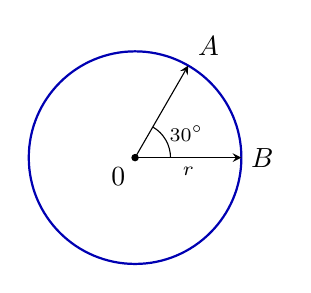
\begin{tikzpicture}[scale=0.9,>=stealth]
  \draw[blue!70!black,thick] (0,0) circle (1.5);
  \fill (0,0) circle (1.5pt) node[below left] {$0$};
  \draw[->] (0,0) -- (0:1.5) node[right] {$B$};
  \draw[->] (0,0) -- (60:1.5) node[above right] {$A$};
  \node[below] at (0.75,0) {\scriptsize $r$};
  \draw (0.5,0) arc (0:60:0.5);
  \node at (25:0.8) {\scriptsize $30^\circ$};
\end{tikzpicture}
\end{center}
\end{example}

\begin{definition}
$1$ រ៉ាដ្យង់ គឺជារង្វាស់មុំផ្ចិតដែលស្កាត់ធ្នូមួយមានប្រវែងស្មើនឹងកាំនៃរង្វង់ ហើយគេកំណត់សរសេរ $1rd$ ។
\end{definition}

យើងដឹងថាប្រវែងធ្នូ $2\pi r$ ស្មើនឹងបរិមាត្ររង្វង់ស្កាត់ដោយមុំ $360^\circ$ ឬមុំ $2\pi$ (rd) មានន័យថា $360^\circ = 2\pi$ (rd) ។ យើងបានទំនាក់ទំនងរវាងរង្វាស់មុំគិតជាដឺក្រេ និងរ៉ាដ្យង់គឺ
\[
\begin{gathered}
1\text{rd} = \frac{180^\circ}{\pi} \approx 57^\circ,\\
1^\circ = \frac{\pi}{180} \approx 0.017 \text{ ។}
\end{gathered}
\]
គេអាចគណនាប្រវែងធ្នូ $AB$ ដោយគ្រាន់តែប្តូរឯកតាមុំដឺក្រេទៅរ៉ាដ្យង់ $\alpha = 30^\circ$ ឬ $\alpha = 30 \times \dfrac{\pi}{180} = 0.52$ rd ប្រវែងធ្នូ $AB = \alpha \cdot r = 0.52 \times 5 = 2.6$ cm ។

\begin{formulaBox}[ជាទូទៅ]
\[ 1\text{rd} = \frac{180^\circ}{\pi}, \quad 1^\circ = \frac{\pi}{180}\text{rd} \text{ ។} \]
\end{formulaBox}

\begin{note}[សម្គាល់]
រង្វាស់មុំគិតជារ៉ាដ្យង់អាចសរសេរដោយមិនប្រើ $rd$ បាន ។ ឧ. $\alpha = \dfrac{\pi}{4}$rd អាចសរសេរដោយខ្លី $\alpha = \dfrac{\pi}{4}$ ។
\end{note}

\begin{example}[លំហាត់គំរូ ៣]
ប្តូរមុំ $30^\circ$, $45^\circ$, $150^\circ$ ជារ៉ាដ្យង់ និងប្តូរមុំ $\dfrac{\pi}{5}$, $\dfrac{2}{3}\pi$, $3\pi$ ជាដឺក្រេ ។
\end{example}
\ans
\[
\begin{gathered}
\frac{\pi}{180} \times 30 = \frac{\pi}{6}, \quad \frac{\pi}{180} \times 45 = \frac{\pi}{4},\\
\frac{\pi}{180} \times 150 = \frac{5\pi}{6}
\end{gathered}
\]
\[
\begin{gathered}
\frac{180^\circ}{\pi} \times \frac{\pi}{5} = 36^\circ, \quad \frac{180^\circ}{\pi} \times \frac{2\pi}{3} = 120^\circ,\\
\frac{180^\circ}{\pi} \times 3\pi = 540^\circ \text{ ។}
\end{gathered}
\]

\begin{pro}
ប្តូរមុំពីរ៉ាដ្យង់ទៅជាដឺក្រេ $\dfrac{4\pi}{3}$, $-\dfrac{4\pi}{3}$, $\dfrac{7\pi}{4}$, $-\dfrac{7\pi}{2}$ ។
\ans
$240^\circ$, \ $-240^\circ$, \ $315^\circ$, \ $-630^\circ$ ។
\end{pro}

\section{អនុគមន៍ត្រីកោណមាត្រ}

\subsection{ស៊ីនុស កូស៊ីនុស តង់សង់ និងកូតង់សង់}

យើងបានសិក្សារួចមកហើយពីផលធៀបត្រីកោណមាត្រ មុំចន្លោះ $0^\circ$ និង $180^\circ$ ក្នុងថ្នាក់ទី $10$ ។ ពេលនេះ យើងកំណត់ $\sin\theta$, $\cos\theta$, $\tan\theta$ និង $\cot\theta$ ដែល $\theta$ ជាមុំទូទៅ ។

ក្នុងរង្វង់ត្រីកោណមាត្រដែលមានផ្ចិត $O$ និងកាំ $r$ ។ $P$ ជាចំណុចមួយនៅលើរង្វង់ដែលមានកូអរដោនេ $P(x, y)$ ហើយមុំ $(\overrightarrow{OA}, \overrightarrow{OP}) = \theta$ ។ $P'$ ជាចំណោលកែងនៃ $P$ លើអ័ក្ស $\overrightarrow{x'x}$ និង $Q$ ជាចំណោលកែងនៃ $P$ លើអ័ក្ស $\overrightarrow{y'y}$ ។
\begin{center}
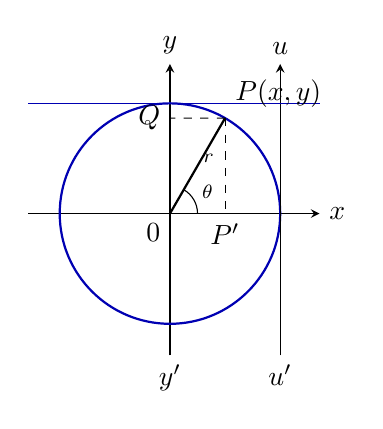
\begin{tikzpicture}[scale=1,>=stealth]
  \draw[->] (-1.8,0) -- (1.9,0) node[right] {$x$};
  \draw[->] (0,-1.8) -- (0,1.9) node[above] {$y$};
  \node[below] at (0,-1.8) {$y'$};
  \draw[blue!70!black,thick] (0,0) circle (1.4);
  \draw[->] (1.4,-1.8) -- (1.4,1.9) node[above] {$u$};
  \node[below] at (1.4,-1.8) {$u'$};
  \draw[blue!70!black] (-1.8,1.4) -- (1.9,1.4);
  \coordinate (P) at (60:1.4);
  \draw[thick] (0,0) -- (P) node[above right] {$P(x, y)$};
  \draw[dashed] (P) -- (P|-0,0) node[below] {$P'$};
  \draw[dashed] (P) -- (0,1.2124) node[left] {$Q$};
  \node[below left] at (0,0) {$0$};
  \draw (0.35,0) arc (0:60:0.35);
  \node at (30:0.55) {\scriptsize $\theta$};
  \node at (55:0.85) {\scriptsize $r$};
\end{tikzpicture}
\end{center}
គេបាន
\[
\begin{gathered}
\sin\theta = \frac{OQ}{OP} = \frac{y}{r}, \quad \cos\theta = \frac{OP'}{OP} = \frac{x}{r},\\
\tan\theta = \frac{\sin\theta}{\cos\theta} = \frac{y}{x}, \quad \cot\theta = \frac{\cos\theta}{\sin\theta} = \frac{x}{y} \text{ ។}
\end{gathered}
\]

\begin{note}[សម្គាល់]
\begin{enumerate}[1]
  \item អ័ក្ស $\overrightarrow{y'y}$ ហៅថាអ័ក្សស៊ីនុស ហើយអ័ក្ស $\overrightarrow{x'x}$ អ័ក្សកូស៊ីនុស ហើយអ័ក្ស $\overrightarrow{u'u}$ ជាអ័ក្សតង់សង់ និងអ័ក្ស $\overrightarrow{v'v}$ ជាអ័ក្សកូតង់សង់ ។
  \item រង្វង់ដែលមានផ្ចិតត្រង់គល់ $O$ មានកាំស្មើ $1$ ហៅថារង្វង់ឯកតា ។
\end{enumerate}
\end{note}

\begin{example}[ឧទាហរណ៍]
គណនាតម្លៃអនុគមន៍ត្រីកោណមាត្រនៃមុំ $\dfrac{\pi}{2}$, $\dfrac{\pi}{6}$ ។

តាមរូប $B$ ជាចំណុចប្រសព្វរវាងរង្វង់និងអ័ក្ស $\overrightarrow{y'y}$ តាមទិសដៅវិជ្ជមាន ។ ដូច្នេះ $B$ ជាចំណុចដែលត្រូវនឹងតម្លៃ $\dfrac{\pi}{2}$ ។
\begin{center}
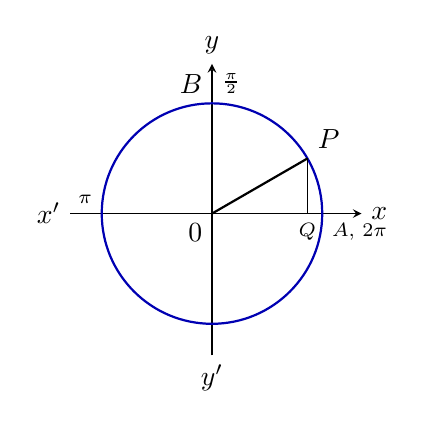
\begin{tikzpicture}[scale=1,>=stealth]
  \draw[->] (-1.8,0) -- (1.9,0) node[right] {$x$};
  \draw[->] (0,-1.8) -- (0,1.9) node[above] {$y$};
  \node[left] at (-1.8,0) {$x'$};
  \node[below] at (0,-1.8) {$y'$};
  \draw[blue!70!black,thick] (0,0) circle (1.4);
  \node[above left] at (0,1.4) {$B$};
  \node[above right] at (0,1.4) {\scriptsize $\frac{\pi}{2}$};
  \node[below right] at (1.4,0) {\scriptsize $A$, $2\pi$};
  \node[above left] at (-1.4,0) {\scriptsize $\pi$};
  \coordinate (P) at (30:1.4);
  \draw[thick] (0,0) -- (P) node[above right] {$P$};
  \draw (P) -- (P|-0,0) node[below] {\scriptsize $Q$};
  \node[below left] at (0,0) {$0$};
\end{tikzpicture}
\end{center}
តាមរូបភាពនេះ គេបាន $\sin\dfrac{\pi}{2} = 1$, $\cos\dfrac{\pi}{2} = 0$ ។
\[
\begin{gathered}
\cot\frac{\pi}{2} = \frac{\cos\frac{\pi}{2}}{\sin\frac{\pi}{2}} = \frac{0}{1} = 0,\\
\tan\frac{\pi}{2} = \frac{\sin\frac{\pi}{2}}{\cos\frac{\pi}{2}} \text{ មិនអាចកំណត់បាន ព្រោះ } \cos\frac{\pi}{2} = 0 \text{ ។}
\end{gathered}
\]
ក្នុងត្រីកោណកែង $OPQ$ គេបាន $\widehat{AOP} = \dfrac{\pi}{6}$ ហើយ $PQ = \dfrac{1}{2}$ ។ ដូច្នេះ
\[
\begin{gathered}
\sin\frac{\pi}{6} = \frac{1}{2}, \quad \cos\frac{\pi}{6} = \sqrt{1 - \frac{1}{4}} = \frac{\sqrt{3}}{2},\\
\tan\frac{\pi}{6} = \frac{\sin\frac{\pi}{6}}{\cos\frac{\pi}{6}} = \frac{\frac{1}{2}}{\frac{\sqrt{3}}{2}} = \frac{1}{\sqrt{3}} = \frac{\sqrt{3}}{3},
\end{gathered}
\]
\[ \cot\frac{\pi}{6} = \frac{\cos\frac{\pi}{6}}{\sin\frac{\pi}{6}} = \frac{\frac{\sqrt{3}}{2}}{\frac{1}{2}} = \sqrt{3} \text{ ។} \]
\end{example}

\begin{formulaBox}[ជាទូទៅ]
គេបានតារាងតម្លៃអនុគមន៍ត្រីកោណមាត្រមុំពិសេស ដូចខាងក្រោម ៖
\[
\renewcommand{\arraystretch}{1.6}
\begin{array}{|c|c|c|c|c|c|c|c|c|c|}\hline
\text{មុំ} & 0 & \frac{\pi}{6} & \frac{\pi}{4} & \frac{\pi}{3} & \frac{\pi}{2} & \frac{2\pi}{3} & \frac{3\pi}{4} & \frac{5\pi}{6} & \pi\\ \hline
\sin & 0 & \frac{1}{2} & \frac{\sqrt{2}}{2} & \frac{\sqrt{3}}{2} & 1 & \frac{\sqrt{3}}{2} & \frac{\sqrt{2}}{2} & \frac{1}{2} & 0\\ \hline
\cos & 1 & \frac{\sqrt{3}}{2} & \frac{\sqrt{2}}{2} & \frac{1}{2} & 0 & -\frac{1}{2} & -\frac{\sqrt{2}}{2} & -\frac{\sqrt{3}}{2} & -1\\ \hline
\tan & 0 & \frac{\sqrt{3}}{3} & 1 & \sqrt{3} & \| & -\sqrt{3} & -1 & -\frac{\sqrt{3}}{3} & 0\\ \hline
\cot & \| & \sqrt{3} & 1 & \frac{\sqrt{3}}{3} & 0 & -\frac{\sqrt{3}}{3} & -1 & -\sqrt{3} & \|\\ \hline
\end{array}
\]
\[
\renewcommand{\arraystretch}{1.6}
\begin{array}{|c|c|c|c|c|c|c|c|c|}\hline
\text{មុំ} & \frac{7\pi}{6} & \frac{5\pi}{4} & \frac{4\pi}{3} & \frac{3\pi}{2} & \frac{5\pi}{3} & \frac{7\pi}{4} & \frac{11\pi}{6} & 2\pi\\ \hline
\sin & -\frac{1}{2} & -\frac{\sqrt{2}}{2} & -\frac{\sqrt{3}}{2} & -1 & -\frac{\sqrt{3}}{2} & -\frac{\sqrt{2}}{2} & -\frac{1}{2} & 0\\ \hline
\cos & -\frac{\sqrt{3}}{2} & -\frac{\sqrt{2}}{2} & -\frac{1}{2} & 0 & \frac{1}{2} & \frac{\sqrt{2}}{2} & \frac{\sqrt{3}}{2} & 1\\ \hline
\tan & \frac{\sqrt{3}}{3} & 1 & \sqrt{3} & \| & -\sqrt{3} & -1 & -\frac{\sqrt{3}}{3} & 0\\ \hline
\cot & \sqrt{3} & 1 & \frac{\sqrt{3}}{3} & 0 & -\frac{\sqrt{3}}{3} & -1 & -\sqrt{3} & \|\\ \hline
\end{array}
\]
(សញ្ញា $\|$ មានន័យថាមិនកំណត់)
\end{formulaBox}

\begin{example}[លំហាត់គំរូ ៤]
គណនា
\begin{enumerate}[a]
  \item $2\sin\dfrac{\pi}{3} + 4\cos\dfrac{\pi}{6} - 3\tan\dfrac{\pi}{3} + 4\cot\dfrac{\pi}{4}$
  \item $\dfrac{5 - 4\tan^2 45^\circ + \cot^2 60^\circ}{2\cos^2 60^\circ - 2\sin^3 90^\circ + 4\tan 45^\circ}$ ។
\end{enumerate}
\end{example}
\ans
\begin{enumerate}[a]
  \item $2 \times \dfrac{\sqrt{3}}{2} + 4 \times \dfrac{\sqrt{3}}{2} - 3 \times \sqrt{3} + 4 \times 1 = \sqrt{3} + 2\sqrt{3} - 3\sqrt{3} + 4 = 4$
  \item $\dfrac{5 - 4 \times 1^2 + \left(\frac{\sqrt{3}}{3}\right)^2}{2 \times \left(\frac{1}{2}\right)^2 - 2 \times 1^3 + 4 \times 1} = \dfrac{1 + \frac{1}{3}}{2 \times \frac{1}{4} - 2 + 4} = \dfrac{8}{15}$ ។
\end{enumerate}

\begin{pro}
គណនា
\begin{enumerate}[a]
  \item $2\sin\dfrac{2\pi}{4} - 3\tan^2\dfrac{\pi}{6} + 2\cos^4\dfrac{\pi}{2} + 3\cot^2\dfrac{\pi}{4}$
  \item $\sin(-135^\circ) + \sin\dfrac{4\pi}{3} + \tan\left(-\dfrac{5\pi}{4}\right)$ ។
\end{enumerate}
\ans
ក. $2 - 1 + 0 + 3 = 4$ \qquad ខ. $-\dfrac{\sqrt{2}}{2} - \dfrac{\sqrt{3}}{2} - 1 = -\dfrac{\sqrt{2} + \sqrt{3} + 2}{2}$ ។
\end{pro}

\subsection{សញ្ញានៃអនុគមន៍ត្រីកោណមាត្រ}

\begin{center}
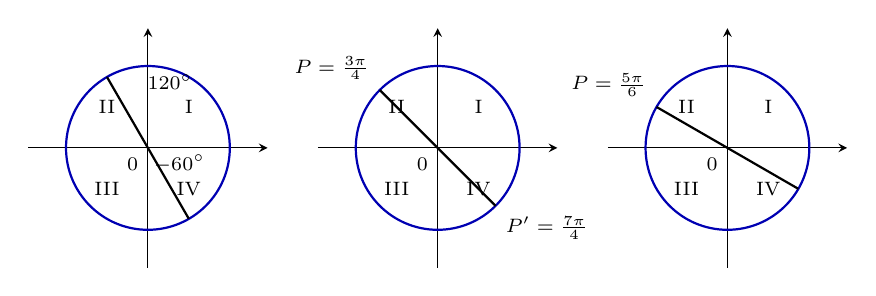
\begin{tikzpicture}[scale=0.8,>=stealth]
  \foreach \k/\a/\lab in {0/120/{},1/135/{},2/150/{}} {
  \begin{scope}[xshift=\k*4.6cm]
    \draw[->] (-1.9,0) -- (1.9,0);
    \draw[->] (0,-1.9) -- (0,1.9);
    \draw[blue!70!black,thick] (0,0) circle (1.3);
    \node at (-0.65,0.65) {\scriptsize II}; \node at (0.65,0.65) {\scriptsize I};
    \node at (-0.65,-0.65) {\scriptsize III}; \node at (0.65,-0.65) {\scriptsize IV};
    \node[below left] at (0,0) {\scriptsize $0$};
  \end{scope}}
  \draw[thick] (0,0) -- (120:1.3); \draw[thick] (0,0) -- (-60:1.3);
  \node at (0.35,1.05) {\scriptsize $120^\circ$}; \node at (0.5,-0.25) {\scriptsize $-60^\circ$};
  \begin{scope}[xshift=4.6cm]
    \draw[thick] (0,0) -- (135:1.3) node[above left] {\scriptsize $P = \frac{3\pi}{4}$};
    \draw[thick] (0,0) -- (-45:1.3) node[below right] {\scriptsize $P' = \frac{7\pi}{4}$};
  \end{scope}
  \begin{scope}[xshift=9.2cm]
    \draw[thick] (0,0) -- (150:1.3) node[above left] {\scriptsize $P = \frac{5\pi}{6}$};
    \draw[thick] (0,0) -- (-30:1.3);
  \end{scope}
\end{tikzpicture}
\end{center}
\[
\begin{gathered}
\cos 120^\circ = -\frac{1}{2}, \quad \sin(-60^\circ) = -\frac{\sqrt{3}}{2},\\
\cos\frac{3\pi}{4} = -\frac{\sqrt{2}}{2},\\
\tan\frac{5\pi}{6} = -\frac{\sqrt{3}}{3}
\end{gathered}
\]
គេបានតារាងសង្ខេបដូចខាងក្រោម ៖
\[
\begin{array}{|c|c|c|c|c|}\hline
\text{អនុគមន៍ \textbackslash\ កាដ្រង់} & \text{I} & \text{II} & \text{III} & \text{IV}\\ \hline
\sin\alpha & + & + & - & -\\ \hline
\cos\alpha & + & - & - & +\\ \hline
\tan\alpha & + & - & + & -\\ \hline
\cot\alpha & + & - & + & -\\ \hline
\end{array}
\]

\begin{example}[លំហាត់គំរូ ៥]
តើមុំ $x$ នៅក្នុងកាដ្រង់ណាដែលផ្ទៀងផ្ទាត់វិសមីការ $\begin{cases} \sin x < 0\\ \cos x < 0 \end{cases}$ ។
\end{example}
\ans
គេបាន $\sin x < 0$ និង $\cos x < 0 \Rightarrow x$ នៅកាដ្រង់ទី III ។ ដូច្នេះ $x$ នៅកាដ្រង់ទី III ។

\begin{pro}
\begin{enumerate}[1]
  \item តើក្នុងកាដ្រង់ណាដែលគេអាចរកមុំផ្ទៀងផ្ទាត់វិសមីការ $\begin{cases} \cos x > 0\\ \tan x > 0 \end{cases}$ ។
  \item
  \begin{enumerate}[a]
    \item តើក្នុងកាដ្រង់ណាដែល $\tan x$ និង $\cot x$ មានសញ្ញាដូចគ្នា?
    \item រកតម្លៃនៃ $\cos\theta$ និង $\tan\theta$ បើ $\sin\theta = -\dfrac{3}{5}$ ដែល $\theta$ នៅកាដ្រង់ទី III ។
  \end{enumerate}
\end{enumerate}
\ans
\begin{enumerate}[1]
  \item (I) ។
  \item ក. គ្រប់កាដ្រង់ (ព្រោះ $\cot x = \dfrac{1}{\tan x}$) \qquad ខ. $\cos\theta = -\dfrac{4}{5}$, \ $\tan\theta = \dfrac{3}{4}$ ។
\end{enumerate}
\end{pro}

\section{លក្ខណៈនៃអនុគមន៍ត្រីកោណមាត្រ}

\subsection{ទំនាក់ទំនងសំខាន់ៗ}

នៅក្នុងរង្វង់ត្រីកោណមាត្រ $\theta$ ជារង្វាស់មុំ $(\overrightarrow{OA}, \overrightarrow{OP})$ គេបាន $\cos\theta = OQ$, $\sin\theta = OR$ ។ ក្នុងត្រីកោណកែង $OPQ$ តាមទ្រឹស្តីបទពីតាគ័រ គេបាន $OP^2 = OQ^2 + PQ^2$
\begin{center}
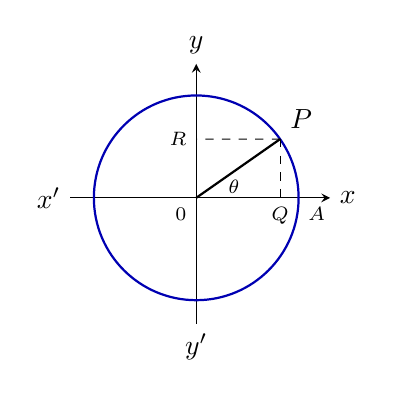
\begin{tikzpicture}[scale=1,>=stealth]
  \draw[->] (-1.6,0) -- (1.7,0) node[right] {$x$};
  \draw[->] (0,-1.6) -- (0,1.7) node[above] {$y$};
  \node[left] at (-1.6,0) {$x'$}; \node[below] at (0,-1.6) {$y'$};
  \draw[blue!70!black,thick] (0,0) circle (1.3);
  \coordinate (P) at (35:1.3);
  \draw[thick] (0,0) -- (P) node[above right] {$P$};
  \draw[dashed] (P) -- (P|-0,0) node[below] {\scriptsize $Q$};
  \draw[dashed] (P) -- (0,0.7457) node[left] {\scriptsize $R$};
  \node[below right] at (1.3,0) {\scriptsize $A$};
  \node[below left] at (0,0) {\scriptsize $0$};
  \node at (17:0.5) {\scriptsize $\theta$};
\end{tikzpicture}
\end{center}
\[ 1 = \sin^2\theta + \cos^2\theta \quad \text{ឬ} \quad \sin^2\theta + \cos^2\theta = 1 \quad (1) \]
ដែល $-1 \le \sin\theta \le 1$, \ $-1 \le \cos\theta \le 1$ ។

គេដឹងថា $\tan\theta = \dfrac{\sin\theta}{\cos\theta}$ ចំពោះ $\cos\theta \ne 0$ គេចែកអង្គទាំងពីរនៃទំនាក់ទំនង $(1)$ និង $\cos^2\theta$ គេបាន
\[ \frac{\sin^2\theta + \cos^2\theta}{\cos^2\theta} = \frac{1}{\cos^2\theta} \quad \text{ឬ} \quad \tan^2\theta + 1 = \frac{1}{\cos^2\theta} \text{ ។} \]
ដូចគ្នាដែរ បើគេចែកទំនាក់ទំនង $(1)$ និង $\sin^2\theta \ne 0$ គេបាន $1 + \cot^2\theta = \dfrac{1}{\sin^2\theta}$ ។

\begin{formulaBox}[គេបានរូបមន្ត]
\[
\begin{gathered}
\sin^2\theta + \cos^2\theta = 1, \quad 1 + \tan^2\theta = \frac{1}{\cos^2\theta},\\
1 + \cot^2\theta = \frac{1}{\sin^2\theta} \text{ ។}
\end{gathered}
\]
\end{formulaBox}

\begin{example}[ឧទាហរណ៍]
គណនា $\cos\theta$, $\tan\theta$, $\cot\theta$ ដោយស្គាល់ $\sin\theta = \dfrac{8}{17}$ និងមុំ $\theta$ នៅកាដ្រង់ទី I ។

គេមាន $\sin^2\theta + \cos^2\theta = 1$ ។ ដោយ $\theta$ នៅកាដ្រង់ទី I នោះ $\cos\theta$ វិជ្ជមាន ។ គេបាន
\[
\begin{gathered}
\cos\theta = \sqrt{1 - \sin^2\theta} = \sqrt{1 - \left(\frac{8}{17}\right)^2} = \sqrt{\frac{225}{289}} = \frac{15}{17},\\
\tan\theta = \frac{\sin\theta}{\cos\theta} = \frac{8}{15}, \quad \cot\theta = \frac{\cos\theta}{\sin\theta} = \frac{15}{8} \text{ ។}
\end{gathered}
\]
\end{example}

\begin{example}[លំហាត់គំរូ ៦]
គណនា $\dfrac{5\sin\alpha + 7\cos\alpha}{6\cos\alpha - 3\sin\alpha}$ ដោយដឹងថា $\tan\alpha = \dfrac{4}{15}$ ។
\end{example}
\ans
\[
\begin{aligned}
\frac{5\sin\alpha + 7\cos\alpha}{6\cos\alpha - 3\sin\alpha} &= \frac{\cos\alpha(5\tan\alpha + 7)}{\cos\alpha(6 - 3\tan\alpha)} = \frac{5 \times \frac{4}{15} + 7}{6 - 3 \times \frac{4}{15}}\\
&= \frac{\frac{4}{3} + 7}{6 - \frac{4}{5}} = \frac{125}{78} \text{ ។}
\end{aligned}
\]

\begin{pro}
\begin{enumerate}[1]
  \item គណនា $\cos\alpha$, $\tan\alpha$, $\cot\alpha$ ដោយគេស្គាល់ $\sin\alpha = -\dfrac{2}{3}$ និង $\dfrac{3\pi}{2} < \alpha < 2\pi$ ។
  \item គណនា $\dfrac{\cot\alpha + \tan\alpha}{\cot\alpha - \tan\alpha}$ ដោយស្គាល់ $\sin\alpha = \dfrac{3}{5}$ និង $0 < \alpha < \dfrac{\pi}{2}$ ។
\end{enumerate}
\ans
\begin{enumerate}[1]
  \item $\cos\alpha = \dfrac{\sqrt{5}}{3}$, \ $\tan\alpha = -\dfrac{2\sqrt{5}}{5}$, \ $\cot\alpha = -\dfrac{\sqrt{5}}{2}$ ។
  \item $\dfrac{25}{7}$ ។
\end{enumerate}
\end{pro}

\subsection{អនុគមន៍ត្រីកោណមាត្រនៃមុំ \texorpdfstring{$\theta$}{θ} និង \texorpdfstring{$\theta + 2k\pi$}{θ + 2kπ}}

ដោយមុំ $\theta$ និង $\theta + 2k\pi$, $k \in \mathbb{Z}$ ជាមុំកំណត់ដោយវ៉ិចទ័រ $\overrightarrow{OA}$ និង $\overrightarrow{OP}$ ដូចគ្នានោះ គេបានរូបមន្ត
\begin{formulaBox}[រូបមន្ត]
\[
\begin{aligned}
\sin(\theta + 2k\pi) &= \sin\theta, & \cos(\theta + 2k\pi) &= \cos\theta\\
\tan(\theta + 2k\pi) &= \tan\theta, & \cot(\theta + 2k\pi) &= \cot\theta \quad (k \in \mathbb{Z})
\end{aligned}
\]
\end{formulaBox}

\begin{note}[សម្គាល់]
$\tan(\theta + k\pi) = \tan\theta$, \ $\cot(\theta + k\pi) = \cot\theta$, \ $k \in \mathbb{Z}$ ។
\end{note}

\begin{example}[ឧទាហរណ៍]
\[
\begin{gathered}
\sin\frac{9}{2}\pi = \sin\left(\frac{\pi}{2} + 4\pi\right) = \sin\frac{\pi}{2} = 1,\\
\cos\left(-\frac{17}{3}\pi\right) = \cos\left(\frac{\pi}{3} - 6\pi\right) = \cos\frac{\pi}{3} = \frac{1}{2} \text{ ។}
\end{gathered}
\]
\end{example}

\begin{example}[លំហាត់គំរូ ៧]
គេដឹងថា $\cos\dfrac{\pi}{4} = \sin\dfrac{\pi}{4} = \dfrac{\sqrt{2}}{2}$ ។ គណនា $\cos\dfrac{65\pi}{4}$ និង $\sin\left(-\dfrac{39\pi}{4}\right)$ ។
\end{example}
\ans
គេសរសេរ $\dfrac{65\pi}{4} = \dfrac{64\pi}{4} + \dfrac{\pi}{4} = 16\pi + \dfrac{\pi}{4}$ ។
\[ \cos\frac{65\pi}{4} = \cos\left[\frac{\pi}{4} + (8 \times 2\pi)\right] = \cos\frac{\pi}{4} = \frac{\sqrt{2}}{2} \text{ ។} \]
គេដឹងថា $-\dfrac{39\pi}{4} = \dfrac{\pi}{4} - \dfrac{40\pi}{4} = \dfrac{\pi}{4} - 10\pi$ គេបាន
\[ \sin\left(-\frac{39\pi}{4}\right) = \sin\left[\frac{\pi}{4} - (5 \times 2\pi)\right] = \sin\frac{\pi}{4} = \frac{\sqrt{2}}{2} \text{ ។} \]

\begin{pro}
គណនាតម្លៃរបស់ $\sin 6\pi$, $\sin\dfrac{11\pi}{3}$, $\cos\left(-\dfrac{23\pi}{6}\right)$, $\tan\left(-\dfrac{27\pi}{4}\right)$ ។
\ans
$0$, \ $-\dfrac{\sqrt{3}}{2}$, \ $\dfrac{\sqrt{3}}{2}$, \ $1$ ។
\end{pro}

\subsection{មុំផ្តុំ}

\textbf{មុំផ្ទុយគ្នា $\theta$ និង $-\theta$}

មុំពីរផ្ទុយគ្នាកាលណាផលបូករង្វាស់វាស្មើនឹងសូន្យតាម $2\pi$ ។ ក្នុងរង្វង់ត្រីកោណមាត្រគេមាន $(\overrightarrow{OA}, \overrightarrow{OP}) = \theta$ និង $(\overrightarrow{OA}, \overrightarrow{OP'}) = \theta'$ ហើយ $\theta + \theta' = 0$ តាម $2\pi$ នាំឱ្យ $\theta' = -\theta$ តាម $2\pi$ ។
\begin{center}
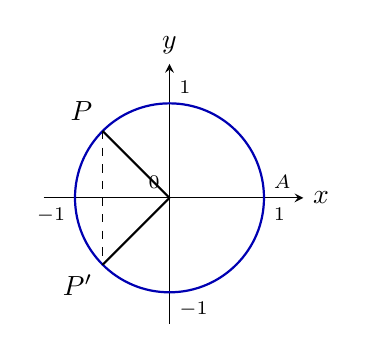
\begin{tikzpicture}[scale=1,>=stealth]
  \draw[->] (-1.6,0) -- (1.7,0) node[right] {$x$};
  \draw[->] (0,-1.6) -- (0,1.7) node[above] {$y$};
  \draw[blue!70!black,thick] (0,0) circle (1.2);
  \draw[thick] (0,0) -- (135:1.2) node[above left] {$P$};
  \draw[thick] (0,0) -- (-135:1.2) node[below left] {$P'$};
  \draw[dashed] (135:1.2) -- (-135:1.2);
  \node[above right] at (1.2,0) {\scriptsize $A$};
  \node[above left] at (0,0) {\scriptsize $0$};
  \node[above right] at (0,1.2) {\scriptsize $1$}; \node[below right] at (0,-1.2) {\scriptsize $-1$};
  \node[below left] at (-1.2,0) {\scriptsize $-1$}; \node[below right] at (1.2,0) {\scriptsize $1$};
\end{tikzpicture}
\end{center}
គេបានកូអរដោនេនៃចំណុច $P$ និង $P'$ គឺ $P(\cos\theta, \sin\theta)$ និង $P'(\cos(-\theta), \sin(-\theta))$ ។ ដោយ $P$ និង $P'$ ឆ្លុះគ្នាធៀបនឹងអ័ក្សអាប់ស៊ីស គេបាន $\sin(-\theta) = -\sin\theta$, $\cos(-\theta) = \cos\theta$ ។ ដូច្នេះ
\[
\begin{gathered}
\tan(-\theta) = \frac{\sin(-\theta)}{\cos(-\theta)} = \frac{-\sin\theta}{\cos\theta} = -\tan\theta,\\
\cot(-\theta) = \frac{\cos(-\theta)}{\sin(-\theta)} = \frac{\cos\theta}{-\sin\theta} = -\cot\theta \text{ ។}
\end{gathered}
\]
\begin{formulaBox}[គេបានរូបមន្ត]
\[
\begin{aligned}
\sin(-\theta) &= -\sin\theta, & \cos(-\theta) &= \cos\theta\\
\tan(-\theta) &= -\tan\theta, & \cot(-\theta) &= -\cot\theta
\end{aligned}
\]
\end{formulaBox}
\begin{note}[សម្គាល់]
មុំពីរផ្ទុយគ្នាមានកូស៊ីនុសដូចគ្នា ហើយមានស៊ីនុស តង់សង់ និងកូតង់សង់ផ្ទុយគ្នា ។ ឧទាហរណ៍ ៖
\[
\begin{gathered}
\sin\left(-\frac{\pi}{3}\right) = -\sin\frac{\pi}{3} = -\frac{\sqrt{3}}{2},\\
\cos\left(-\frac{\pi}{3}\right) = \cos\frac{\pi}{3} = \frac{1}{2},\\
\cot\left(-\frac{\pi}{3}\right) = -\cot\frac{\pi}{3} = -\frac{\sqrt{3}}{3} \text{ ។}
\end{gathered}
\]
\end{note}

\textbf{មុំបំពេញ $\left(\frac{\pi}{2} - \theta\right)$ និង $\theta$}

មុំពីរបំពេញគ្នា កាលណាផលបូករង្វាស់វាស្មើនឹង $\dfrac{\pi}{2}$ តាម $2\pi$ ។

ក្នុងរង្វង់ត្រីកោណ គេមាន $(\overrightarrow{OA}, \overrightarrow{OP}) = \theta$ និង $(\overrightarrow{OA}, \overrightarrow{OP'}) = \dfrac{\pi}{2} - \theta$ ។ គេបានកូអរដោនេនៃចំណុច $P$ គឺ $(\cos\theta, \sin\theta)$ ។ បើគេយកចំណុច $P'$ ឆ្លុះគ្នានឹងចំណុច $P$ ធៀបនឹងបន្ទាត់ $y = x$ នោះគេបាន កូអរដោនេនៃចំណុច $P'$ គឺ $(\sin\theta, \cos\theta)$ \ $(1)$ ។
\begin{center}
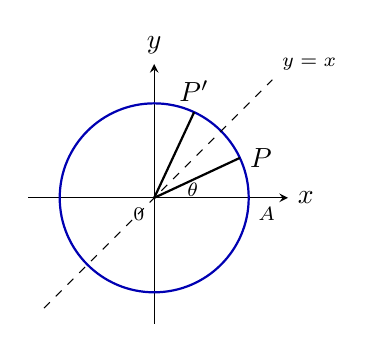
\begin{tikzpicture}[scale=1,>=stealth]
  \draw[->] (-1.6,0) -- (1.7,0) node[right] {$x$};
  \draw[->] (0,-1.6) -- (0,1.7) node[above] {$y$};
  \draw[blue!70!black,thick] (0,0) circle (1.2);
  \draw[dashed] (-1.4,-1.4) -- (1.5,1.5) node[above right] {\scriptsize $y = x$};
  \draw[thick] (0,0) -- (25:1.2) node[right] {$P$};
  \draw[thick] (0,0) -- (65:1.2) node[above] {$P'$};
  \node[below right] at (1.2,0) {\scriptsize $A$};
  \node[below left] at (0,0) {\scriptsize $0$};
  \node at (12:0.5) {\scriptsize $\theta$};
\end{tikzpicture}
\end{center}
តាមរូបខាងស្តាំ $OP'$ ជាជ្រុងមួយនៃមុំ $\left(\dfrac{\pi}{2} - \theta\right)$ ។ ដូច្នេះកូអរដោនេនៃ $P'$ គឺ $\left[\cos\left(\dfrac{\pi}{2} - \theta\right), \sin\left(\dfrac{\pi}{2} - \theta\right)\right]$ \ $(2)$ ។
តាម $(1)$ និង $(2)$ គេបាន
\[ \sin\left(\frac{\pi}{2} - \theta\right) = \cos\theta \quad \text{និង} \quad \cos\left(\frac{\pi}{2} - \theta\right) = \sin\theta \]
\[
\begin{gathered}
\tan\left(\frac{\pi}{2} - \theta\right) = \frac{\sin\left(\frac{\pi}{2} - \theta\right)}{\cos\left(\frac{\pi}{2} - \theta\right)} = \frac{\cos\theta}{\sin\theta} = \cot\theta = \frac{1}{\tan\theta},\\
\cot\left(\frac{\pi}{2} - \theta\right) = \frac{\cos\left(\frac{\pi}{2} - \theta\right)}{\sin\left(\frac{\pi}{2} - \theta\right)} = \frac{\sin\theta}{\cos\theta} = \tan\theta \text{ ។}
\end{gathered}
\]
\begin{note}[សម្គាល់]
\begin{itemize}
  \item មុំពីរបំពេញគ្នា មានចុងឆ្លុះគ្នាធៀបនឹងបន្ទាត់ពុះទី $1$ ។ គេបានរូបមន្ត
  \[
  \begin{aligned}
  \sin\left(\frac{\pi}{2} - \theta\right) &= \cos\theta, & \cos\left(\frac{\pi}{2} - \theta\right) &= \sin\theta\\
  \tan\left(\frac{\pi}{2} - \theta\right) &= \cot\theta, & \cot\left(\frac{\pi}{2} - \theta\right) &= \tan\theta
  \end{aligned}
  \]
  \item មុំពីរបំពេញគ្នា មានស៊ីនុសនៃមុំមួយស្មើនឹងកូស៊ីនុសនៃមុំមួយទៀត ហើយតង់សង់នៃមុំមួយស្មើនឹងកូតង់សង់នៃមុំមួយទៀត ។ ឧទាហរណ៍ ៖
  \[
\begin{gathered}
\sin 60^\circ = \cos(90^\circ - 60^\circ) = \cos 30^\circ = \frac{\sqrt{3}}{2},\\
\tan\frac{\pi}{3} = \tan\left(\frac{\pi}{2} - \frac{\pi}{6}\right) = \cot\frac{\pi}{6} = \sqrt{3} \text{ ។}
\end{gathered}
\]
\end{itemize}
\end{note}

\textbf{មុំបន្ថែម $(\pi - \theta)$ និង $\theta$}

មុំពីរបន្ថែមគ្នា កាលណាផលបូករង្វាស់វាស្មើនឹង $\pi$ តាម $2\pi$ ។

ក្នុងរង្វង់ត្រីកោណមាត្រ គេមានមុំ $(\overrightarrow{OA}, \overrightarrow{OP}) = \theta$ និងមុំ $(\overrightarrow{OA}, \overrightarrow{OP'}) = \pi - \theta$ ។ គេបានកូអរដោនេនៃចំណុច $P$ គឺ $(\cos\theta, \sin\theta)$ និងកូអរដោនេនៃចំណុច $P'(-\cos\theta, \sin\theta)$ \ $(1)$ ។ តាមរូបខាងស្តាំ $OP'$ ជាជ្រុងមួយនៃមុំ $(\pi - \theta)$ ។ ដូច្នេះកូអរដោនេនៃ $P'$ គឺ $(\cos(\pi - \theta), \sin(\pi - \theta))$ \ $(2)$ ។
\begin{center}
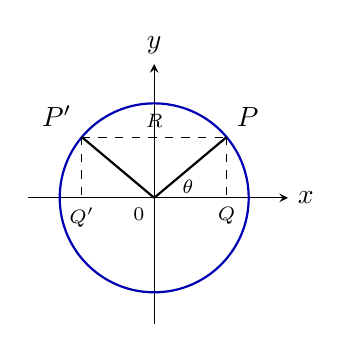
\begin{tikzpicture}[scale=1,>=stealth]
  \draw[->] (-1.6,0) -- (1.7,0) node[right] {$x$};
  \draw[->] (0,-1.6) -- (0,1.7) node[above] {$y$};
  \draw[blue!70!black,thick] (0,0) circle (1.2);
  \coordinate (P) at (40:1.2); \coordinate (Pp) at (140:1.2);
  \draw[thick] (0,0) -- (P) node[above right] {$P$};
  \draw[thick] (0,0) -- (Pp) node[above left] {$P'$};
  \draw[dashed] (Pp) -- (P);
  \draw[dashed] (P) -- (P|-0,0) node[below] {\scriptsize $Q$};
  \draw[dashed] (Pp) -- (Pp|-0,0) node[below] {\scriptsize $Q'$};
  \node[above] at (0,0.77) {\scriptsize $R$};
  \node[below left] at (0,0) {\scriptsize $0$};
  \node at (18:0.45) {\scriptsize $\theta$};
\end{tikzpicture}
\end{center}
តាម $(1)$ និង $(2)$ គេបាន
\[ \sin(\pi - \theta) = \sin\theta, \quad \cos(\pi - \theta) = -\cos\theta \]
\[
\begin{gathered}
\tan(\pi - \theta) = \frac{\sin(\pi - \theta)}{\cos(\pi - \theta)} = \frac{\sin\theta}{-\cos\theta} = -\tan\theta,\\
\cot(\pi - \theta) = \frac{\cos(\pi - \theta)}{\sin(\pi - \theta)} = \frac{-\cos\theta}{\sin\theta} = -\cot\theta
\end{gathered}
\]
មុំពីរបន្ថែមមានចុងឆ្លុះគ្នាធៀបនឹងអ័ក្សស៊ីនុសគេបានរូបមន្ត
\begin{formulaBox}[រូបមន្ត]
\[
\begin{aligned}
\sin(\pi - \theta) &= \sin\theta, & \cos(\pi - \theta) &= -\cos\theta\\
\tan(\pi - \theta) &= -\tan\theta, & \cot(\pi - \theta) &= -\cot\theta
\end{aligned}
\]
\end{formulaBox}
\begin{note}[សម្គាល់]
មុំពីរបន្ថែមគ្នា មានស៊ីនុសដូចគ្នាហើយមានកូស៊ីនុស តង់សង់ និងកូតង់សង់ផ្ទុយគ្នា ។
\end{note}
\begin{example}[ឧទាហរណ៍]
\[ \sin 135^\circ = \sin(180^\circ - 45^\circ) = \sin 45^\circ = \frac{\sqrt{2}}{2} \]
\[
\begin{aligned}
\cos\left(-\frac{20\pi}{3}\right) &= \cos\frac{20\pi}{3} = \cos\left(\frac{2\pi}{3} + 6\pi\right) = \cos\frac{2\pi}{3}\\
&= \cos\left(\pi - \frac{\pi}{3}\right) = -\cos\frac{\pi}{3} = -\frac{1}{2} \text{ ។}
\end{aligned}
\]
\end{example}

\begin{example}[លំហាត់គំរូ ៨]
គណនាតម្លៃលេខនៃកន្សោម ៖
\[
\begin{gathered}
A = \cos(-\theta) + \sin\left(\frac{\pi}{2} - \theta\right) + \cos(\pi - \theta) + \sin\left(\frac{3}{2}\pi + \theta\right),\\
B = \sin\frac{5\pi}{6} + \cos\frac{3\pi}{4} + \sin\left(-\frac{\pi}{6}\right) \text{ ។}
\end{gathered}
\]
\end{example}
\ans
\[ A = \cos\theta + \cos\theta - \cos\theta - \cos\theta = 0 \]
\[
\begin{aligned}
B &= \sin\frac{5\pi}{6} + \cos\frac{3\pi}{4} + \sin\left(-\frac{\pi}{6}\right)\\
&= \sin\left(\pi - \frac{\pi}{6}\right) + \cos\left(\pi - \frac{\pi}{4}\right) - \sin\frac{\pi}{6}\\
&= \sin\frac{\pi}{6} - \cos\frac{\pi}{4} - \sin\frac{\pi}{6} = -\cos\frac{\pi}{4} = -\frac{\sqrt{2}}{2} \text{ ។}
\end{aligned}
\]

\begin{pro}
\begin{enumerate}[1]
  \item ដោយស្គាល់ $\sin 47^\circ = 0.6820$ គណនា $\cos 43^\circ$ ។
  \item រកតម្លៃលេខនៃកន្សោម
  \[
\begin{gathered}
A = \sin(-x) + \sin(\pi - x) + \cos(\pi - x) + \sin\left(\frac{\pi}{2} - x\right),\\
B = \sin\left(\frac{5\pi}{2} - x\right) + \cos(3\pi - x),\\
C = \tan\frac{5\pi}{6} + \cot\frac{7\pi}{4} + \frac{1}{\tan\frac{\pi}{3}} \text{ ។}
\end{gathered}
\]
\end{enumerate}
\ans
\begin{enumerate}[1]
  \item $\cos 43^\circ = \sin 47^\circ = 0.6820$ ។
  \item $A = 0$, \ $B = 0$, \ $C = -1$ ។
\end{enumerate}
\end{pro}

\textbf{មុំដែលមានផលសងស្មើ $\pi$}

ក្នុងរង្វង់ត្រីកោណមាត្រ គេមានមុំ $(\overrightarrow{OA}, \overrightarrow{OP}) = \theta$ និងមុំ $(\overrightarrow{OA}, \overrightarrow{OP'}) = \pi + \theta$ គេបានកូអរដោនេនៃចំណុច $P(\cos\theta, \sin\theta)$ និងកូអរដោនេនៃចំណុច $P'(\cos(\pi + \theta), \sin(\pi + \theta))$ ។ ចំណុច $P$ និង $P'$ ឆ្លុះគ្នាធៀបនឹងគល់ $O$ ។ គេបាន $OP$ និង $OP'$ មានចំណោលកែងផ្ទុយគ្នាលើអ័ក្សស៊ីនុស និងអ័ក្សកូស៊ីនុស ។
\begin{center}
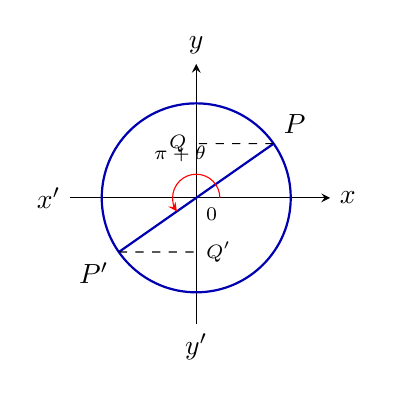
\begin{tikzpicture}[scale=1,>=stealth]
  \draw[->] (-1.6,0) -- (1.7,0) node[right] {$x$};
  \draw[->] (0,-1.6) -- (0,1.7) node[above] {$y$};
  \node[left] at (-1.6,0) {$x'$}; \node[below] at (0,-1.6) {$y'$};
  \draw[blue!70!black,thick] (0,0) circle (1.2);
  \draw[blue!70!black,thick] (35:1.2) node[above right,black] {$P$} -- (215:1.2) node[below left,black] {$P'$};
  \draw[dashed] (35:1.2) -- (0,0.688) node[left] {\scriptsize $Q$};
  \draw[dashed] (215:1.2) -- (0,-0.688) node[right] {\scriptsize $Q'$};
  \draw[red,->] (0.3,0) arc (0:215:0.3);
  \node at (110:0.6) {\scriptsize $\pi + \theta$};
  \node[below right] at (0,0) {\scriptsize $0$};
\end{tikzpicture}
\end{center}
គេបាន
\[
\begin{aligned}
\sin(\pi + \theta) &= \sin[\pi - (-\theta)] = \sin(-\theta) = -\sin\theta\\
\cos(\pi + \theta) &= \cos[\pi - (-\theta)] = -\cos(-\theta) = -\cos\theta\\
\tan(\pi + \theta) &= \frac{\sin(\pi + \theta)}{\cos(\pi + \theta)} = \frac{-\sin\theta}{-\cos\theta} = \tan\theta\\
\cot(\pi + \theta) &= \frac{\cos(\pi + \theta)}{\sin(\pi + \theta)} = \frac{-\cos\theta}{-\sin\theta} = \cot\theta \text{ ។}
\end{aligned}
\]
\begin{formulaBox}[គេបានរូបមន្ត]
\[
\begin{aligned}
\sin(\pi + \theta) &= -\sin\theta, & \cos(\pi + \theta) &= -\cos\theta\\
\tan(\pi + \theta) &= \tan\theta, & \cot(\pi + \theta) &= \cot\theta
\end{aligned}
\]
\end{formulaBox}
\begin{example}[ឧទាហរណ៍]
\[
\begin{gathered}
\sin 210^\circ = \sin(180^\circ + 30^\circ) = -\sin 30^\circ = -\frac{1}{2},\\
\tan\frac{7\pi}{6} = \tan\left(\pi + \frac{\pi}{6}\right) = \tan\frac{\pi}{6} = \frac{\sqrt{3}}{3}
\end{gathered}
\]
\[
\begin{aligned}
A &= 2\cos(\pi - 2x) + \sin(\pi + y) - 2\cos(\pi - 2x)\\
&\quad - \sin(\pi + y)\\
&= -2\cos 2x - \sin y + 2\cos 2x + \sin y = 0 \text{ ។}
\end{aligned}
\]
\end{example}

\textbf{មុំដែលមានផលសងស្មើ $\frac{\pi}{2}$}

ក្នុងរង្វង់ត្រីកោណមាត្រ គេមានមុំ $(\overrightarrow{OA}, \overrightarrow{OP}) = \theta$ និងមុំ $(\overrightarrow{OA}, \overrightarrow{OP'}) = \dfrac{\pi}{2} + \theta = \dfrac{\pi}{2} - (-\theta)$ ។ ធ្នូ $AP'$ ជាធ្នូបំពេញនៃធ្នូដែលមានរង្វាស់ $(-\theta)$ តាម $2\pi$ ។ ដូច្នេះ
\begin{formulaBox}[រូបមន្ត]
\[
\begin{aligned}
\sin\left(\theta + \frac{\pi}{2}\right) &= \cos(-\theta)\\
&= \cos\theta, & \cos\left(\theta + \frac{\pi}{2}\right) &= \sin(-\theta)\\
&= -\sin\theta\\
\tan\left(\theta + \frac{\pi}{2}\right) &= \cot(-\theta)\\
&= -\cot\theta, & \cot\left(\theta + \frac{\pi}{2}\right) &= \tan(-\theta)\\
&= -\tan\theta
\end{aligned}
\]
\end{formulaBox}
\begin{example}[ឧទាហរណ៍]
\[
\begin{gathered}
\sin 120^\circ = \sin(30^\circ + 90^\circ) = \cos 30^\circ = \frac{\sqrt{3}}{2},\\
\tan\frac{5\pi}{6} = \tan\left(\frac{\pi}{2} + \frac{\pi}{3}\right) = -\cot\frac{\pi}{3} = -\frac{\sqrt{3}}{3}
\end{gathered}
\]
\[ \frac{\cot\frac{3}{4}\pi}{\sin\frac{3}{2}\pi} = \frac{\cot\left(\frac{\pi}{2} + \frac{\pi}{4}\right)}{\sin\left(\frac{\pi}{2} + \pi\right)} = \frac{-\tan\frac{\pi}{4}}{\cos\pi} = \frac{-1}{-1} = 1 \text{ ។} \]
\end{example}

\begin{example}[លំហាត់គំរូ ៩]
គណនា $\dfrac{\cos(-288^\circ)\cot 72^\circ}{\tan(-162^\circ)\sin 108^\circ} - \tan 18^\circ$ ។
\end{example}
\ans
\[
\begin{aligned}
&\frac{\cos(-288^\circ)\cot 72^\circ}{\tan(-162^\circ)\sin 108^\circ} - \tan 18^\circ\\
&= \frac{\cos(-360^\circ + 72^\circ)\cot 72^\circ}{\tan(-180^\circ + 18^\circ)\sin(90^\circ + 18^\circ)}\\
&\quad - \tan 18^\circ\\
&= \frac{\cos 72^\circ \tan 18^\circ}{\tan 18^\circ \cos 18^\circ} - \tan 18^\circ\\
&= \frac{\cos(90^\circ - 18^\circ)\tan 18^\circ}{\tan 18^\circ \cos 18^\circ} - \tan 18^\circ\\
&= \frac{\sin 18^\circ}{\cos 18^\circ} - \tan 18^\circ = \tan 18^\circ - \tan 18^\circ = 0 \text{ ។}
\end{aligned}
\]

\begin{pro}
\begin{enumerate}[1]
  \item គណនា $\sin 870^\circ$, $\cos(-135^\circ)$, $\tan 765^\circ$, $\cot\dfrac{25}{4}\pi$ ។
  \item គណនា $\dfrac{(\cot 44^\circ + \tan 226^\circ)\cos 406^\circ}{\cos 316^\circ} - \cot 72^\circ\cot 18^\circ$ ។
\end{enumerate}
\ans
\begin{enumerate}[1]
  \item $\dfrac{1}{2}$, \ $-\dfrac{\sqrt{2}}{2}$, \ $1$, \ $1$ ។
  \item $\tan 44^\circ$ ។
\end{enumerate}
\end{pro}

\section{ការសិក្សាអនុគមន៍ត្រីកោណមាត្រ}

ដើម្បីសិក្សាអនុគមន៍ត្រីកោណមាត្រ គេត្រូវរកដែនកំណត់ ខួប ភាពគូសេស ទិសដៅអថេរភាពនិងក្រាបនៃអនុគមន៍ ។

\subsection{ដែនកំណត់}

អនុគមន៍ស៊ីនុសនិងអនុគមន៍កូស៊ីនុសមានដែនកំណត់លើ $\mathbb{R}$ ។ អនុគមន៍តង់សង់អាចកំណត់បាន លុះត្រាតែ $\cos x \ne 0 \Rightarrow x \ne \dfrac{\pi}{2} + k\pi$, $k \in \mathbb{Z}$ ។ ដូច្នេះដែនកំណត់នៃអនុគមន៍តង់សង់គឺ $D = \mathbb{R} - \left\{\dfrac{\pi}{2} + k\pi\right\}$, $k \in \mathbb{Z}$ ។

អនុគមន៍កូតង់សង់អាចកំណត់បាន លុះត្រាតែ $\sin x \ne 0 \Rightarrow x \ne k\pi$, $k \in \mathbb{Z}$ ។ ដូច្នេះដែនកំណត់នៃអនុគមន៍កូតង់សង់គឺ $D = \mathbb{R} - \{k\pi\}$, $k \in \mathbb{Z}$ ។

\begin{example}[ឧទាហរណ៍]
អនុគមន៍ $y = \sin 2x$ មានដែនកំណត់ $D = \mathbb{R}$ ។

អនុគមន៍ $y = \dfrac{4}{\cos x}$ កំណត់បាន កាលណា $\cos x \ne 0 \Rightarrow x \ne \dfrac{\pi}{2} + k\pi$ ។

អនុគមន៍ $y = \tan(x - 1)$ កំណត់បានកាលណា $x - 1 \ne \dfrac{\pi}{2} + k\pi$, $x \ne 1 + \dfrac{\pi}{2} + k\pi$, $k \in \mathbb{Z}$ ។
\end{example}

\subsection{ខួបនៃអនុគមន៍}

\begin{definition}
$f$ ជាអនុគមន៍មានដែនកំណត់ $D$ ។ $f$ ជាអនុគមន៍មានខួប $p$ លុះត្រាតែ $p$ ជាចំនួនវិជ្ជមានតូចបំផុត ដែល $\forall x \in D$ ៖ $f(x + p) = f(x)$ ។ ពីនិយមន័យនេះគេអាចទាញបាន
\[ f(x) = f(x + p) = f[(x + p) + p] = f(x + 2p) = \ldots \]
\[ f(x) = f(x - p) = f[(x - p) - p] = f(x - 2p) = \ldots \]
\end{definition}

\begin{formulaBox}[ជាទូទៅ]
អនុគមន៍ស៊ីនុសនិងកូស៊ីនុសមានខួប $2\pi$ ព្រោះ $2\pi$ ជាចំនួនវិជ្ជមានតូចបំផុតដែល $\sin(x + 2\pi) = \sin x$ និង $\cos(x + 2\pi) = \cos x$ ដែល $\forall k \in \mathbb{Z}$, $\forall x \in D$, $f(x + kp) = f(x)$ ។
\end{formulaBox}

\begin{note}[សម្គាល់]
អនុគមន៍ $y = \sin 2x$ និង $y = \cos 2x$ មានខួប $\pi$ ព្រោះ $\sin[2(x + \pi)] = \sin(2x + 2\pi) = \sin 2x$ និង $\cos[2(x + \pi)] = \cos(2x + 2\pi) = \cos 2x$ ។
\end{note}

\begin{formulaBox}[ជាទូទៅ]
អនុគមន៍ $y = \sin ax$ និង $y = \cos ax$ មានខួប $p = \dfrac{2\pi}{|a|}$ ។
\end{formulaBox}

អនុគមន៍តង់សង់និងអនុគមន៍កូតង់សង់មានខួប $\pi$ ព្រោះ $\forall x \in \mathbb{R}$, $\forall k \in \mathbb{Z}$, $\tan(x + \pi) = \tan x$ នាំឱ្យ $\tan(x + k\pi) = \tan x$ និង $\cot(x + \pi) = \cot x$ នាំឱ្យ $\cot(x + k\pi) = \cot x$ ។

\begin{formulaBox}[ជាទូទៅ]
អនុគមន៍ $y = \tan ax$ និង $y = \cot ax$ មានខួប $p = \dfrac{\pi}{|a|}$ ។
\end{formulaBox}

\begin{example}[ឧទាហរណ៍]
អនុគមន៍ $y = \sin\dfrac{1}{2}x$ មានខួប $p = 4\pi$, \ $y = \cos(-3x)$ មានខួប $p = \dfrac{2\pi}{|-3|} = \dfrac{2\pi}{3}$ ។

អនុគមន៍ $y = 3\tan\dfrac{1}{2}x$ មានខួប $p = 2\pi$, \ $y = \cot 5x$ មានខួប $p = \dfrac{\pi}{5}$ ។
\end{example}

\subsection{ភាពគូនិងភាពសេស}

\begin{definition}
\begin{itemize}
  \item $f$ ជាអនុគមន៍មានដែនកំណត់ $D$ ។ $f$ ជាអនុគមន៍គូ លុះត្រាតែគ្រប់ $x \in D$, $-x \in D$, $f(-x) = f(x)$ ។
  \item $f$ ជាអនុគមន៍មានដែនកំណត់ $D$ ។ $f$ ជាអនុគមន៍សេស លុះត្រាតែគ្រប់ $x \in D$, $-x \in D$, $f(-x) = -f(x)$ ។
\end{itemize}
\end{definition}

\begin{example}[ឧទាហរណ៍]
$y = x - \sin x$ មានដែនកំណត់ $D = \mathbb{R}$ ។ គ្រប់តម្លៃ $x \in D$, $-x \in D$, $f(-x) = -x - \sin(-x) = -(x - \sin x) = -f(x)$ ។ ដូច្នេះ $y = x - \sin x$ ជាអនុគមន៍សេស ។

$y = \tan x\cot^3 x$ មានដែនកំណត់ $D = \mathbb{R} - \left\{\dfrac{k\pi}{2}\right\}$, $k \in \mathbb{Z}$ ។ គ្រប់តម្លៃ $x \in D$, $-x \in D$, $f(-x) = \tan(-x)\cot^3(-x) = \tan x\cot^3 x = f(x)$ ។ ដូច្នេះ $y = \tan x\cot^3 x$ ជាអនុគមន៍គូ ។
\end{example}

\textbf{លក្ខណៈ} ក្រាបនៃអនុគមន៍សេសមានគល់តម្រុយជាផ្ចិតឆ្លុះ និងក្រាបនៃអនុគមន៍គូមានអ័ក្សអរដោនេជាអ័ក្សឆ្លុះ ។

\subsection{អថេរភាពនិងក្រាបនៃអនុគមន៍ \texorpdfstring{$y = \sin x$}{y = sin x}}

\textbf{ដែនកំណត់} ៖ $y = \sin x$ ជាអនុគមន៍ កំណត់ចំពោះគ្រប់ $x \in \mathbb{R}$ ។

\textbf{ខួប} ៖ $y = \sin x$ ជាអនុគមន៍ខួបដែលមានខួប $p = 2\pi$ ព្រោះ $\sin(x + 2\pi) = \sin x$ ។ យើងសិក្សាអនុគមន៍ $y = \sin x$ លើ $[-\pi, \pi]$ ហើយក្រាបនៃអនុគមន៍ $y = \sin x$ លើចន្លោះ $[(2k - 1)\pi, (2k + 1)\pi]$ បានដោយរំកិលមែកលើ $[-\pi, \pi]$ ចំនួន $2\pi$ តាមអ័ក្ស $(x'x)$ ។

\textbf{ភាពសេស} ៖ គេដឹងថា $\sin(-x) = -\sin x$ ។ ដូច្នេះអនុគមន៍ $y = \sin x$ ជាអនុគមន៍សេស ។ ក្រាបនៃអនុគមន៍ $y = \sin x$ មានគល់តម្រុយជាផ្ចិតឆ្លុះ ។ ដូច្នេះសិក្សាអនុគមន៍ $y = \sin x$ តែលើ $[0, \pi]$ រួចធ្វើបម្លែងឆ្លុះធៀបនឹង $0$ បានមែកលើ $[-\pi, 0]$ ។

\textbf{ទិសដៅអថេរភាព} ៖ គេសង្កេតឃើញថា កាលណា $x$ កើនពី $0$ ទៅ $\dfrac{\pi}{2}$ នោះតម្លៃ $\sin x$ កើនពី $0$ ទៅ $1$ ។ បើ $x$ កើនពី $\dfrac{\pi}{2}$ ទៅ $\pi$ នោះតម្លៃ $\sin x$ ចុះពី $1$ ទៅ $0$ ។

\textbf{តារាងអថេរភាពនិងក្រាប $y = \sin x$ លើ $[-\pi, \pi]$}
\begin{center}
\begin{tikzpicture}
  \tkzTabInit[lgt=1.6,espcl=2]{$x$ /1, $\sin x$ /1.6}{$0$, $\frac{\pi}{2}$, $\pi$}
  \tkzTabVar{-/$0$, +/$1$, -/$0$}
\end{tikzpicture}

\begin{tikzpicture}[scale=0.9,>=stealth]
  \draw[->] (-4,0) -- (4.2,0) node[right] {$x$};
  \draw[->] (0,-1.4) -- (0,1.6) node[above] {$y$};
  \draw[green!50!black,thick,domain=-3.1416:3.1416,samples=80] plot (\x,{sin(\x r)});
  \draw[dotted] (-4,1) -- (4,1); \draw[dotted] (-4,-1) -- (4,-1);
  \node[below] at (3.1416,0) {\scriptsize $\pi$}; \node[above] at (-3.1416,0) {\scriptsize $-\pi$};
  \node[below] at (1.5708,0) {\scriptsize $\frac{\pi}{2}$}; \node[above] at (-1.5708,0) {\scriptsize $-\frac{\pi}{2}$};
  \node[left] at (0,1.15) {\scriptsize $1$}; \node[right] at (0,-1.15) {\scriptsize $-1$};
  \node[below left] at (0,0) {\scriptsize $0$};
\end{tikzpicture}
\end{center}
ក្រាបនេះហៅថា \textbf{ស៊ីនុសូអ៊ីត} ។

\begin{example}[ឧទាហរណ៍]
សិក្សាអថេរភាពនិងសង់ក្រាបនៃអនុគមន៍ $y = 2\sin x$ លើចន្លោះ $[0, 2\pi]$ ។

\textbf{ដែនកំណត់} ៖ អនុគមន៍ $y = 2\sin x$ មានដែនកំណត់ $D = \mathbb{R}$ ។ អនុគមន៍ $y = 2\sin x$ មានខួប $p = 2\pi$ ។

\textbf{ភាពសេស} ៖ គ្រប់ $x \in D$, $-x \in D$, $f(-x) = 2\sin(-x) = -2\sin x = -f(x)$ ។ ដូច្នេះ $y = 2\sin x$ ជាអនុគមន៍សេស ។

\textbf{តារាងអថេរភាពនិងក្រាប}
\begin{center}
\begin{tikzpicture}
  \tkzTabInit[lgt=1.6,espcl=1.6]{$x$ /1, $2\sin x$ /1.8}{$0$, $\frac{\pi}{2}$, $\pi$, $\frac{3\pi}{2}$, $2\pi$}
  \tkzTabVar{-/$0$, +/$2$, R/, -/$-2$, +/$0$}
  \tkzTabVal{2}{4}{0.5}{}{$0$}
\end{tikzpicture}

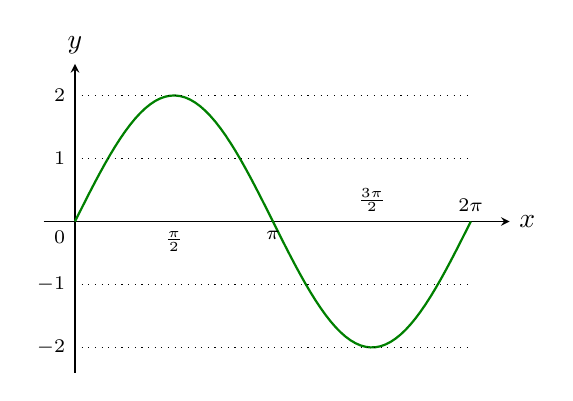
\begin{tikzpicture}[scale=0.8,>=stealth]
  \draw[->] (-0.5,0) -- (6.9,0) node[right] {$x$};
  \draw[->] (0,-2.4) -- (0,2.5) node[above] {$y$};
  \draw[green!50!black,thick,domain=0:6.2832,samples=80] plot (\x,{2*sin(\x r)});
  \draw[dotted] (0,2) -- (6.3,2); \draw[dotted] (0,-2) -- (6.3,-2); \draw[dotted] (0,1) -- (6.3,1); \draw[dotted] (0,-1) -- (6.3,-1);
  \foreach \y in {-2,-1,1,2} \node[left] at (0,\y) {\scriptsize $\y$};
  \node[below] at (1.5708,0) {\scriptsize $\frac{\pi}{2}$}; \node[below] at (3.1416,0) {\scriptsize $\pi$};
  \node[above] at (4.7124,0) {\scriptsize $\frac{3\pi}{2}$}; \node[above] at (6.2832,0) {\scriptsize $2\pi$};
  \node[below left] at (0,0) {\scriptsize $0$};
\end{tikzpicture}
\end{center}
\end{example}

\begin{example}[លំហាត់គំរូ ១០]
ដោយប្រើក្រាបនៃអនុគមន៍ $y = \sin x$ ។ សង់ក្រាបនៃអនុគមន៍ $y = \sin\left(x + \dfrac{\pi}{2}\right)$ ។
\end{example}
\ans
ក្រាបនៃអនុគមន៍ $y = \sin\left(x + \dfrac{\pi}{2}\right)$ សង់បានដោយរំកិលក្រាបនៃអនុគមន៍ $y = \sin x$ ពីស្តាំទៅឆ្វេងចំនួន $\dfrac{\pi}{2}$ ឯកតាតាមអ័ក្ស $x'x$ ។
\begin{center}
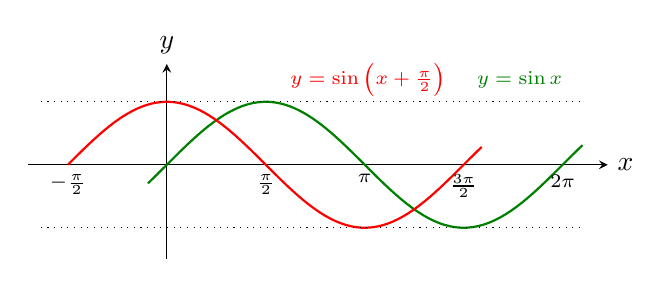
\begin{tikzpicture}[scale=0.8,>=stealth]
  \draw[->] (-2.2,0) -- (7,0) node[right] {$x$};
  \draw[->] (0,-1.5) -- (0,1.6) node[above] {$y$};
  \draw[green!50!black,thick,domain=-0.3:6.6,samples=80] plot (\x,{sin(\x r)});
  \draw[red,thick,domain=-1.5708:5,samples=80] plot (\x,{sin((\x+1.5708) r)});
  \draw[dotted] (-2,1) -- (6.6,1); \draw[dotted] (-2,-1) -- (6.6,-1);
  \node[below] at (-1.5708,0) {\scriptsize $-\frac{\pi}{2}$};
  \node[below] at (1.5708,0) {\scriptsize $\frac{\pi}{2}$}; \node[below] at (3.1416,0) {\scriptsize $\pi$};
  \node[below] at (4.7124,0) {\scriptsize $\frac{3\pi}{2}$}; \node[below] at (6.2832,0) {\scriptsize $2\pi$};
  \node[green!50!black] at (5.6,1.35) {\scriptsize $y = \sin x$};
  \node[red] at (3.2,1.35) {\scriptsize $y = \sin\left(x + \frac{\pi}{2}\right)$};
\end{tikzpicture}
\end{center}

\begin{pro}
\begin{enumerate}[1]
  \item សិក្សាអថេរភាពនិងសង់ក្រាបនៃអនុគមន៍ $y = \sin 2x$ ។
  \item ប្រើក្រាប $y = \sin x$ សង់ក្រាប $y = \sin\left(x - \dfrac{\pi}{3}\right)$ ។
\end{enumerate}
\end{pro}

\subsection{អថេរភាពនិងក្រាបនៃអនុគមន៍ \texorpdfstring{$y = \cos x$}{y = cos x}}

\textbf{ដែនកំណត់} ៖ កូស៊ីនុសជាអនុគមន៍ កំណត់ចំពោះគ្រប់ $x \in \mathbb{R}$ ។

\textbf{ខួប} ៖ $y = \cos x$ ជាអនុគមន៍ដែលមានខួប $p = 2\pi$ ។ យើងសិក្សាអនុគមន៍ $y = \cos x$ លើចន្លោះ $[(2k - 1)\pi, (2k + 1)\pi]$, $k \in \mathbb{Z}$ បានដោយរំកិលមែកលើ $[-\pi, \pi]$ ចំនួន $2\pi$ តាម $(x'x)$ ។

\textbf{ភាពគូ} ៖ គេដឹងថា $\cos(-x) = \cos x$ ដូច្នេះ $y = \cos x$ ជាអនុគមន៍គូ ។ ក្រាបនៃ $y = \cos x$ មានអ័ក្សអរដោនេជាអ័ក្សឆ្លុះ ។ ដូច្នេះ យើងសិក្សាតែលើ $[0, \pi]$ ហើយមែកលើ $[-\pi, 0]$ បានដោយធ្វើបម្លែងឆ្លុះធៀបនឹងអ័ក្សអរដោនេនៃមែកលើ $[0, \pi]$ ។

\textbf{ទិសដៅអថេរភាព} ៖ គេសង្កេតឃើញថាកាលណា $x$ កើនពី $0$ ទៅ $\dfrac{\pi}{2}$ នោះតម្លៃ $\cos x$ ចុះពី $1$ ទៅ $0$ ។ បើ $x$ កើនពី $\dfrac{\pi}{2}$ ទៅ $\pi$ នោះតម្លៃ $\cos x$ ចុះពី $0$ ទៅ $-1$ ។

\textbf{តារាងអថេរភាពនិងក្រាប $y = \cos x$}
\begin{center}
\begin{tikzpicture}
  \tkzTabInit[lgt=1.6,espcl=2]{$x$ /1, $\cos x$ /1.8}{$0$, $\frac{\pi}{2}$, $\pi$}
  \tkzTabVar{+/$1$, R/, -/$-1$}
  \tkzTabVal{1}{3}{0.5}{}{$0$}
\end{tikzpicture}

\begin{tikzpicture}[scale=0.9,>=stealth]
  \draw[->] (-4,0) -- (4.2,0) node[right] {$x$};
  \draw[->] (0,-1.4) -- (0,1.6) node[above] {$y$};
  \draw[green!50!black,thick,domain=-3.1416:3.1416,samples=80] plot (\x,{cos(\x r)});
  \draw[dotted] (-4,1) -- (4,1); \draw[dotted] (-4,-1) -- (4,-1);
  \node[above] at (3.1416,0) {\scriptsize $\pi$}; \node[above] at (-3.1416,0) {\scriptsize $-\pi$};
  \node[below] at (1.5708,0) {\scriptsize $\frac{\pi}{2}$}; \node[below] at (-1.5708,0) {\scriptsize $-\frac{\pi}{2}$};
  \node[above right] at (0,1) {\scriptsize $1$}; \node[right] at (0,-1.15) {\scriptsize $-1$};
  \node[below left] at (0,0) {\scriptsize $0$};
\end{tikzpicture}
\end{center}

\begin{example}[ឧទាហរណ៍]
សិក្សាអថេរភាពនិងសង់ក្រាបនៃអនុគមន៍ $y = 2\cos x$ ។

\textbf{ដែនកំណត់} ៖ អនុគមន៍ $y = 2\cos x$ មានដែនកំណត់ $D = \mathbb{R}$ ។ អនុគមន៍ $y = 2\cos x$ មានខួប $T = 2\pi$ ។

$x \in D$, $-x \in D$, $f(-x) = 2\cos(-x) = 2\cos x = f(x)$ ។ ដូច្នេះ $y = 2\cos x$ ជាអនុគមន៍គូ ។

\textbf{តារាងអថេរភាពនិងក្រាប}
\begin{center}
\begin{tikzpicture}
  \tkzTabInit[lgt=1.6,espcl=1.6]{$x$ /1, $2\cos x$ /1.8}{$-\pi$, $-\frac{\pi}{2}$, $0$, $\frac{\pi}{2}$, $\pi$}
  \tkzTabVar{-/$-2$, R/, +/$2$, R/, -/$-2$}
  \tkzTabVal{1}{3}{0.5}{}{$0$}
  \tkzTabVal{3}{5}{0.5}{}{$0$}
\end{tikzpicture}

\begin{tikzpicture}[scale=0.8,>=stealth]
  \draw[->] (-4,0) -- (4.2,0) node[right] {$x$};
  \draw[->] (0,-2.4) -- (0,2.6) node[above] {$y$};
  \draw[green!50!black,thick,domain=-3.1416:3.1416,samples=80] plot (\x,{2*cos(\x r)});
  \draw[dotted] (-3.5,2) -- (3.5,2); \draw[dotted] (-3.5,-2) -- (3.5,-2);
  \node[above] at (3.1416,0) {\scriptsize $\pi$}; \node[above] at (-3.1416,0) {\scriptsize $-\pi$};
  \node[below] at (1.5708,0) {\scriptsize $\frac{\pi}{2}$}; \node[below] at (-1.5708,0) {\scriptsize $-\frac{\pi}{2}$};
  \node[above right] at (0,2) {\scriptsize $2$}; \node[right] at (0,-2.15) {\scriptsize $-2$};
  \node[below left] at (0,0) {\scriptsize $0$};
\end{tikzpicture}
\end{center}
\end{example}

\begin{example}[លំហាត់គំរូ ១១]
ដោយប្រើក្រាបនៃអនុគមន៍ $y = \cos x$ សង់ក្រាបនៃអនុគមន៍ $y = \cos\left(x - \dfrac{\pi}{2}\right)$ ។
\end{example}
\ans
គេបានក្រាបនៃអនុគមន៍ $y = \cos\left(x - \dfrac{\pi}{2}\right)$ ដោយរំកិលក្រាបនៃអនុគមន៍ $y = \cos x$ ពីឆ្វេងទៅស្តាំ $\dfrac{\pi}{2}$ ឯកតាស្របនឹងអ័ក្ស $(x'x)$ ។
\begin{center}
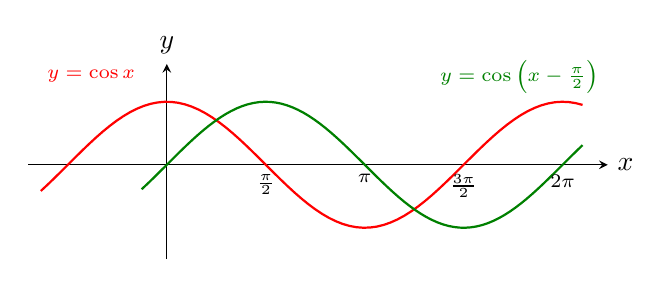
\begin{tikzpicture}[scale=0.8,>=stealth]
  \draw[->] (-2.2,0) -- (7,0) node[right] {$x$};
  \draw[->] (0,-1.5) -- (0,1.6) node[above] {$y$};
  \draw[red,thick,domain=-2:6.6,samples=80] plot (\x,{cos(\x r)});
  \draw[green!50!black,thick,domain=-0.4:6.6,samples=80] plot (\x,{cos((\x-1.5708) r)});
  \node[below] at (1.5708,0) {\scriptsize $\frac{\pi}{2}$}; \node[below] at (3.1416,0) {\scriptsize $\pi$};
  \node[below] at (4.7124,0) {\scriptsize $\frac{3\pi}{2}$}; \node[below] at (6.2832,0) {\scriptsize $2\pi$};
  \node[green!50!black] at (5.6,1.4) {\scriptsize $y = \cos\left(x - \frac{\pi}{2}\right)$};
  \node[red] at (-1.2,1.4) {\scriptsize $y = \cos x$};
\end{tikzpicture}
\end{center}

\begin{pro}
សិក្សាអថេរភាពនិងសង់ក្រាបនៃអនុគមន៍ $y = \cos 2x$ និង $y = \cos\left(x - \dfrac{\pi}{6}\right)$ ។
\end{pro}

\subsection{អថេរភាពនិងក្រាបនៃអនុគមន៍ \texorpdfstring{$y = \tan x$}{y = tan x}}

\textbf{ដែនកំណត់} ៖ គេដឹងថា $\tan x = \dfrac{\sin x}{\cos x}$ ។ អនុគមន៍តង់សង់កំណត់ចំពោះគ្រប់ $x \in \mathbb{R}$ ខុសពី $\dfrac{\pi}{2} + k\pi$, $(k \in \mathbb{Z})$ ឬ $x \in \mathbb{R} - \left\{\dfrac{\pi}{2} + k\pi\right\}$, $(k \in \mathbb{Z})$ ។

\textbf{ខួប} ៖ $y = \tan x$ ជាអនុគមន៍ដែលមានខួប $p = \pi$ ។ យើងសិក្សាអនុគមន៍ $y = \tan x$ លើចន្លោះ $\left((2k - 1)\dfrac{\pi}{2}, (2k + 1)\dfrac{\pi}{2}\right)$, $(k \in \mathbb{Z})$ បានដោយរំកិលមែកលើ $\left(-\dfrac{\pi}{2}, \dfrac{\pi}{2}\right)$ ចំនួន $\pi$ ឯកតាតាម $(x'x)$ ។

\textbf{ភាពសេស} ៖ គេដឹងថាគ្រប់ $x \ne \left(\dfrac{\pi}{2} + k\pi\right)$, $(k \in \mathbb{Z})$ នាំឱ្យ $\tan(-x) = -\tan x$ ។ ដូច្នេះ $y = \tan x$ ជាអនុគមន៍សេស ។ ក្រាបនៃ $y = \tan x$ មានគល់តម្រុយជាផ្ចិតឆ្លុះ ។ ដូច្នេះយើងសិក្សាតែលើ $\left[0, \dfrac{\pi}{2}\right)$ ហើយមែកលើ $\left(-\dfrac{\pi}{2}, 0\right]$ បានដោយធ្វើបម្លែងឆ្លុះធៀបនឹង $0$ នៃមែកលើ $\left[0, \dfrac{\pi}{2}\right)$ ។

\textbf{ទិសដៅអថេរភាព} ៖ គេសង្កេតឃើញថាអនុគមន៍ $y = \tan x$ កើនលើចន្លោះ $\left[0, \dfrac{\pi}{2}\right)$ ។

\textbf{តារាងអថេរភាពនិងក្រាប}
\begin{center}
\begin{tikzpicture}
  \tkzTabInit[lgt=1.6,espcl=3]{$x$ /1, $\tan x$ /1.6}{$0$, $\frac{\pi}{2}$}
  \tkzTabVar{-/$0$, +D/$+\infty$}
\end{tikzpicture}

\begin{tikzpicture}[scale=0.75,>=stealth]
  \draw[->] (-5.2,0) -- (5.4,0) node[right] {$x$};
  \draw[->] (0,-3.2) -- (0,3.4) node[above] {$y$};
  \foreach \c in {-3.1416,0,3.1416} \draw[green!50!black,thick,domain=\c-1.25:\c+1.25,samples=60] plot (\x,{tan((\x-\c) r)});
  \foreach \a in {-4.7124,-1.5708,1.5708,4.7124} \draw[red,dotted] (\a,-3.2) -- (\a,3.2);
  \node[below] at (-4.7124,0) {\scriptsize $-\frac{3\pi}{2}$}; \node[above left] at (-3.1416,0) {\scriptsize $-\pi$};
  \node[above left] at (-1.5708,0) {\scriptsize $-\frac{\pi}{2}$}; \node[above right] at (1.5708,0) {\scriptsize $\frac{\pi}{2}$};
  \node[above right] at (3.1416,0) {\scriptsize $\pi$}; \node[below] at (4.7124,0) {\scriptsize $\frac{3\pi}{2}$};
  \node[green!50!black] at (4.2,3) {\scriptsize $y = \tan x$};
\end{tikzpicture}
\end{center}

\begin{example}[ឧទាហរណ៍]
សិក្សាអថេរភាពនិងសង់ក្រាបនៃអនុគមន៍ $y = \dfrac{1}{2}\tan x$ ។

\textbf{ដែនកំណត់} ៖ អនុគមន៍ $y = \dfrac{1}{2}\tan x$ មានដែនកំណត់ $D = \mathbb{R} - \left\{\dfrac{\pi}{2} + k\pi\right\}$ $(k \in \mathbb{Z})$ ។

\textbf{ខួប} ៖ អនុគមន៍ $y = \dfrac{1}{2}\tan x$ មានខួប $p = \pi$ ។ គេដឹងថាគ្រប់ $x \ne \left(\dfrac{\pi}{2} + k\pi\right)$, $(k \in \mathbb{Z})$ នាំឱ្យ $\dfrac{1}{2}\tan(-x) = -\dfrac{1}{2}\tan x = -f(x)$ ជាអនុគមន៍សេស ។

\textbf{តារាងអថេរភាពនិងក្រាប}
\begin{center}
\[
\renewcommand{\arraystretch}{1.6}
\begin{array}{|c|ccccccccc|}\hline
x & -\frac{\pi}{2} & & -\frac{\pi}{4} & & 0 & & \frac{\pi}{4} & & \frac{\pi}{2}\\ \hline
\frac{1}{2}\tan x & \| -\infty & \nearrow & -\frac{1}{2} & \nearrow & 0 & \nearrow & \frac{1}{2} & \nearrow & +\infty \|\\ \hline
\end{array}
\]

\begin{tikzpicture}[scale=0.9,>=stealth]
  \draw[->] (-2.2,0) -- (2.3,0) node[right] {$x$};
  \draw[->] (0,-2.6) -- (0,2.8) node[above] {$y$};
  \draw[green!50!black,thick,domain=-1.36:1.36,samples=60] plot (\x,{0.5*tan(\x r)});
  \draw[dotted] (-1.5708,-2.6) -- (-1.5708,2.6); \draw[dotted] (1.5708,-2.6) -- (1.5708,2.6);
  \node[below] at (-0.7854,0) {\scriptsize $-\frac{\pi}{4}$}; \node[below] at (0.7854,0) {\scriptsize $\frac{\pi}{4}$};
  \node[below left] at (0,0) {\scriptsize $0$};
  \node[green!50!black] at (1.1,2.6) {\scriptsize $y = \frac{1}{2}\tan x$};
\end{tikzpicture}
\end{center}
\end{example}

\begin{example}[លំហាត់គំរូ ១២]
សង់ក្រាបនៃអនុគមន៍ $y = \tan\left(\dfrac{\pi}{6} - x\right)$ ។
\end{example}
\ans
តាង $X = x - \dfrac{\pi}{6}$, $x = X + \dfrac{\pi}{6}$, $y = -\tan X$ ។ តារាងអថេរភាពនិងក្រាប
\[
\renewcommand{\arraystretch}{1.6}
\begin{array}{|c|c|c|c|c|c|}\hline
X & -\frac{\pi}{2} & -\frac{\pi}{4} & 0 & \frac{\pi}{4} & \frac{\pi}{2}\\ \hline
x = X + \frac{\pi}{6} & -\frac{\pi}{3} & -\frac{\pi}{12} & \frac{\pi}{6} & \frac{5\pi}{12} & \frac{2\pi}{3}\\ \hline
y & \| \ +\infty \searrow & 1 \searrow & 0 & \searrow -1 & \searrow -\infty \ \|\\ \hline
\end{array}
\]
\begin{center}
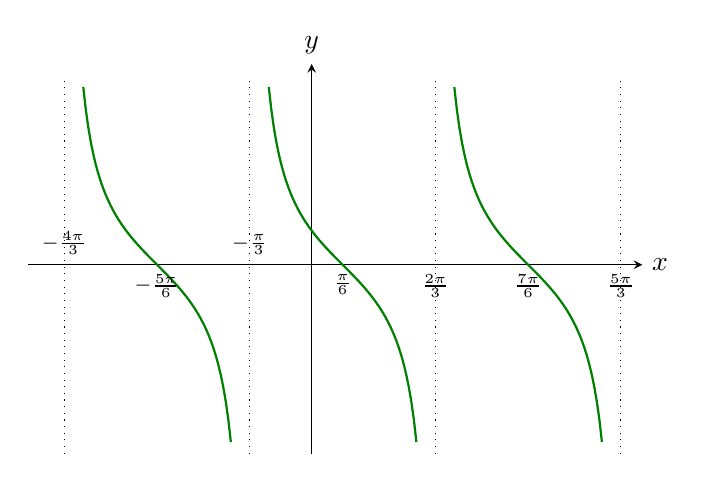
\begin{tikzpicture}[scale=0.75,>=stealth]
  \draw[->] (-4.8,0) -- (5.6,0) node[right] {$x$};
  \draw[->] (0,-3.2) -- (0,3.4) node[above] {$y$};
  \foreach \c in {-2.618,0.5236,3.6652} \draw[green!50!black,thick,domain=\c-1.25:\c+1.25,samples=60] plot (\x,{-tan((\x-\c) r)});
  \foreach \a in {-4.1888,-1.0472,2.0944,5.236} \draw[dotted] (\a,-3.2) -- (\a,3.2);
  \node[above] at (-4.1888,0) {\scriptsize $-\frac{4\pi}{3}$}; \node[above] at (-1.0472,0) {\scriptsize $-\frac{\pi}{3}$};
  \node[below] at (0.5236,0) {\scriptsize $\frac{\pi}{6}$}; \node[below] at (2.0944,0) {\scriptsize $\frac{2\pi}{3}$};
  \node[below] at (-2.618,0) {\scriptsize $-\frac{5\pi}{6}$}; \node[below] at (3.6652,0) {\scriptsize $\frac{7\pi}{6}$};
  \node[below] at (5.236,0) {\scriptsize $\frac{5\pi}{3}$};
\end{tikzpicture}
\end{center}

\begin{pro}
សង់ក្រាបនៃអនុគមន៍ $y = \dfrac{1}{2}\tan 2x$ និង $y = \tan\left(x - \dfrac{\pi}{6}\right)$ ។
\end{pro}

\subsection{អថេរភាពនិងក្រាបនៃអនុគមន៍ \texorpdfstring{$y = \cot x$}{y = cot x}}

\textbf{ដែនកំណត់} ៖ គេដឹងថា $\cot x = \dfrac{\cos x}{\sin x}$ ។ ដូច្នេះ អនុគមន៍កូតង់សង់កំណត់និងជាប់ចំពោះគ្រប់ $x \ne k\pi$ $(k \in \mathbb{Z})$ ។

\textbf{ខួប} ៖ $y = \cot x$ ជាអនុគមន៍ដែលមានខួប $p = \pi$ ។ យើងសិក្សាអនុគមន៍ $y = \cot x$ លើចន្លោះ $(k\pi, (k + 1)\pi)$, $(k \in \mathbb{Z})$ បានដោយរំកិលមែកលើ $(0, \pi)$ ចំនួន $\pi$ ឯកតាតាម $(x'x)$ ។

\textbf{ភាពសេស} ៖ ដោយ $\cot(-x) = -\cot x$ នាំឱ្យ $y = \cot x$ ជាអនុគមន៍សេស ។ ក្រាបនៃ $y = \cot x$ មានគល់ $0$ ជាផ្ចិតឆ្លុះ ។ យើងសិក្សាអនុគមន៍ $y = \cot x$ លើចន្លោះ $\left(0, \dfrac{\pi}{2}\right]$ ។

\textbf{ទិសដៅអថេរភាព} ៖ អនុគមន៍ $y = \cot x$ ចុះលើចន្លោះ $\left(0, \dfrac{\pi}{2}\right]$ ។

\textbf{តារាងអថេរភាពនិងក្រាប}
\begin{center}
\begin{tikzpicture}
  \tkzTabInit[lgt=1.6,espcl=3]{$x$ /1, $\cot x$ /1.6}{$0$, $\frac{\pi}{2}$}
  \tkzTabVar{D+/$+\infty$, -/$0$}
\end{tikzpicture}

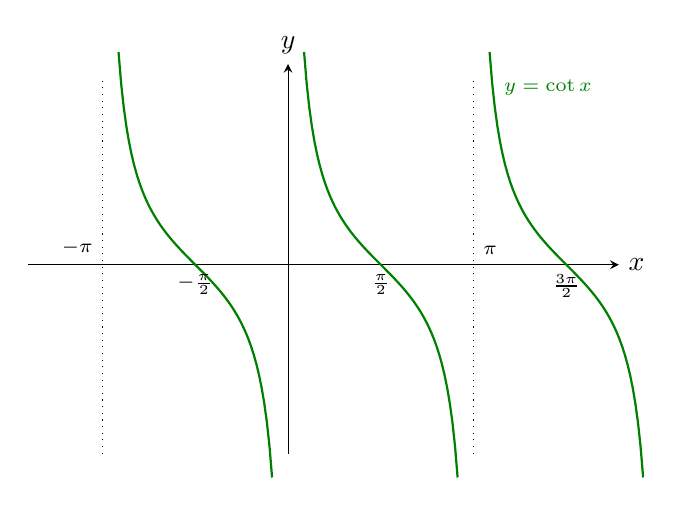
\begin{tikzpicture}[scale=0.75,>=stealth]
  \draw[->] (-4.4,0) -- (5.6,0) node[right] {$x$};
  \draw[->] (0,-3.2) -- (0,3.4) node[above] {$y$};
  \foreach \c in {-1.5708,1.5708,4.7124} \draw[green!50!black,thick,domain=\c-1.3:\c+1.3,samples=60] plot (\x,{-tan((\x-\c) r)});
  \foreach \a in {-3.1416,3.1416} \draw[dotted] (\a,-3.2) -- (\a,3.2);
  \node[above left] at (-3.1416,0) {\scriptsize $-\pi$}; \node[below] at (-1.5708,0) {\scriptsize $-\frac{\pi}{2}$};
  \node[below] at (1.5708,0) {\scriptsize $\frac{\pi}{2}$}; \node[above right] at (3.1416,0) {\scriptsize $\pi$};
  \node[below] at (4.7124,0) {\scriptsize $\frac{3\pi}{2}$};
  \node[green!50!black] at (4.4,3) {\scriptsize $y = \cot x$};
\end{tikzpicture}
\end{center}

\begin{pro}
សង់ក្រាបនៃអនុគមន៍ $y = \dfrac{1}{2}\cot x$ ។
\end{pro}

\section*{លំហាត់អនុវត្តន៍}
\begin{enumerate}[1]
  \item បំប្លែងជារ៉ាដ្យង់នៃមុំ $200^\circ$, $-100^\circ$, $225^\circ$, $-240^\circ$, $-135^\circ$, $330^\circ$, $570^\circ$, $630^\circ$ ។
  \item បំប្លែងជាដឺក្រេនៃមុំ $\dfrac{2\pi}{3}$, $\dfrac{5\pi}{4}$, $\dfrac{5\pi}{6}$, $\dfrac{5\pi}{7}$, $\dfrac{7\pi}{4}$, $-\dfrac{11\pi}{6}$, $-\dfrac{5\pi}{2}$, $-\dfrac{7\pi}{2}$, $\dfrac{\pi}{9}$ ។
  \item គេមាន $\sin\theta + \cos\theta = -\dfrac{1}{2}$ ហើយ $\pi < \theta < 2\pi$ ។ គណនា
  \begin{tasks}(3)
    \task $\sin\theta\cos\theta$
    \task $\tan\theta + \dfrac{1}{\tan\theta}$
    \task $\sin^3\theta + \cos^3\theta$ ។
  \end{tasks}
  \item រកតម្លៃកន្សោមខាងក្រោម ៖
  \begin{enumerate}[a]
    \item $A = \dfrac{8\cos^3\alpha - 2\sin^3\alpha + \cos\alpha}{2\cos\alpha - \sin^3\alpha}$ ដោយស្គាល់ $\tan\alpha = 2$ ។
    \item $B = \dfrac{\sin\alpha + \cos\alpha}{\cos\alpha - \sin\alpha}$ ដោយស្គាល់ $\tan\alpha = -2$ ។
    \item $C = \dfrac{\sin^2\alpha - \cos^2\alpha}{\sin^2\alpha - 2\cos^2\alpha}$ ដោយស្គាល់ $\cot\alpha = 3$ ។
  \end{enumerate}
  \item សម្រួលកន្សោមខាងក្រោម ៖
  \begin{tasks}(2)
    \task $\sqrt{\tan^2\alpha + \cot^2\alpha + 2}$
    \task $\dfrac{\sin^2\alpha - \tan^2\alpha}{\cos^2\alpha - \cot^2\alpha}$
    \task $\sqrt{\sin^2\alpha(1 + \cot\alpha) + \cos^2\alpha(1 + \tan\alpha)}$
    \task $\dfrac{\cos^2\alpha + \cos^2\alpha\cot^2\alpha}{\sin^2\alpha + \sin^2\alpha\tan^2\alpha}$ ។
  \end{tasks}
  \item ផ្ទៀងផ្ទាត់សមភាពខាងក្រោម ៖
  \begin{tasks}(2)
    \task $\dfrac{\sin x + \cos x - 1}{\sin x - \cos x + 1} = \dfrac{\cos x}{1 + \sin x}$
    \task $\dfrac{\cos x\cot x - \sin x\tan x}{\frac{1}{\sin x} - \frac{1}{\cos x}} = 1 + \sin x\cos x$
    \task $(\tan\theta - \sin\theta)^2 + (1 - \cos\theta)^2 = \left(\dfrac{1}{\cos\theta} - 1\right)^2$
    \task $\dfrac{2\sin\theta\cos\theta - \cos\theta}{1 - \sin\theta + \sin^2\theta - \cos^2\theta} = \dfrac{1}{\tan\theta}$ ។
  \end{tasks}
  \item រកខួបនៃអនុគមន៍ខាងក្រោម ៖
  \begin{tasks}(3)
    \task $y = \sin\dfrac{2}{3}x$
    \task $y = -\sin\dfrac{1}{4}x$
    \task $y = 2\cos\dfrac{1}{4}x$
    \task $y = \tan\dfrac{1}{4}x$
    \task $y = \cot\dfrac{1}{3}x$
    \task $y = \sin 2x + \cos x$ ។
  \end{tasks}
  \item រកភាពគូនិងសេសនៃអនុគមន៍ត្រីកោណមាត្រខាងក្រោម ៖
  \begin{tasks}(3)
    \task $y = x - \sin 2x$
    \task $y = x^2\cos^2 x$
    \task $y = \tan x\cos^2 x$
    \task* $y = \sin 5x + \sin 3x + 5\sin x\cos 2x$ \ $(x \in \mathbb{R})$
    \task* $y = \sin x + \tan x + \cot 3x$ \ $\left(x \ne \dfrac{k\pi}{2}\right)$
    \task* $y = \cos x + \sin\dfrac{x}{2}\sin x + 5x^2$ ។
  \end{tasks}
  \item សង់ក្រាបនៃអនុគមន៍ខាងក្រោម ៖
  \begin{tasks}(4)
    \task $y = -\sin\dfrac{x}{3}$
    \task $y = -\sin\theta + 1$
    \task $y = \cos\left(\theta + \dfrac{\pi}{4}\right)$
    \task $y = 3\tan\theta$ ។
  \end{tasks}
  \item ដោយប្រើក្រាប $y = \sin x$ សង់ក្រាបនៃអនុគមន៍ខាងក្រោម ៖
  \begin{tasks}(3)
    \task $y = \sin\left(x + \dfrac{\pi}{3}\right)$
    \task $y = 2 + \sin x$
    \task $y = 1 - \sin x$ ។
  \end{tasks}
  \item ដោយប្រើក្រាប $y = \cos x$ សង់ក្រាបនៃអនុគមន៍ ៖
  \begin{tasks}(3)
    \task $y = \cos\left(x + \dfrac{\pi}{2}\right)$
    \task $y = 2 - \cos x$
    \task $y = \cos x + 2$ ។
  \end{tasks}
  \item គេមានត្រីកោណកែងដែលមានអ៊ីប៉ូតេនុស $1$ និងជ្រុងឈរមុំ $\beta$ ស្មើ $p$ ពោលគឺ $\sin\beta = p$ ហើយ $\beta$ ជាមុំស្រួច ។ ចូរគណនាកន្សោមខាងក្រោមជាអនុគមន៍នៃ $p$ ៖
  \begin{tasks}(3)
    \task $\tan\beta$
    \task $\sin(90^\circ - \beta)$
    \task $\sin(180^\circ + \beta)$ ។
  \end{tasks}
  \item គេមាន $QRS$ ជាបន្ទាត់ត្រង់ ហើយ $PQ = 12$ cm, $QR = 5$ cm និង $RP = 13$ cm ($RS = 5$ cm) ។
  \begin{center}
  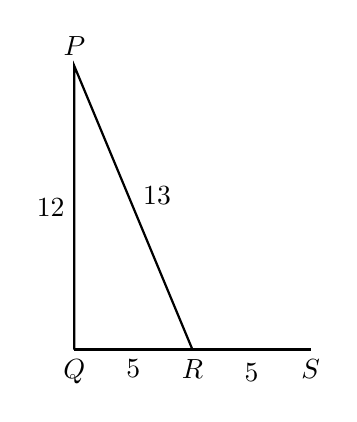
\begin{tikzpicture}[scale=0.3]
    \draw[thick] (0,0) node[below] {$Q$} -- (5,0) node[below] {$R$} -- (10,0) node[below] {$S$};
    \draw[thick] (0,0) -- (0,12) node[above] {$P$} -- (5,0);
    \node[left] at (0,6) {$12$}; \node[right] at (2.5,6.5) {$13$}; \node[below] at (2.5,0) {$5$}; \node[below] at (7.5,-0.2) {$5$};
  \end{tikzpicture}
  \end{center}
  \begin{enumerate}[a]
    \item ពន្យល់ថាហេតុអ្វីបានជា $\angle PQR$ ជាមុំកែង ។
    \item ទាញរកតម្លៃ $\angle QPR$ និង $\cos\angle PRS$ ។
  \end{enumerate}
  \item បង្ហាញថា $\cos\theta\left(\dfrac{1}{1 - \sin\theta} - \dfrac{1}{1 + \sin\theta}\right)$ អាចសរសេរក្នុងទម្រង់ $k\tan\theta$ និងរកតម្លៃនៃ $k$ ។
\end{enumerate}
